%%%%%%%%%%%%%%%%%%%%%%%%%%%
%                         %
%       2014.11.21.       %
%      TDK dolgozat       %
%    Tamás     LATEX      %
%%%%%%%%%%%%%%%%%%%%%%%%%%%
\documentclass[oneside,titlepage,12pt,a4paper]{report}
%\documentclass[12pt]{report}
\usepackage[centertags]{amsmath}
\usepackage{amsfonts}
\usepackage{amsthm}
\usepackage{newlfont}
%\usepackage[ansinew]{inputenc}
\usepackage[magyar]{babel}	
\usepackage[utf8]{inputenc}		
\usepackage{t1enc}				
\usepackage{graphicx}
\usepackage{color}
%\usepackage[colorlinks]{hyperref}
%\usepackage[active,new,noold,marker]{xrcs}
\usepackage{euler}
\usepackage{amssymb,latexsym}
\usepackage{amsmath}
\usepackage{graphics}
\usepackage{algorithm} 
\usepackage{algpseudocode} %ezzel összeakadhat \usepackage{algorithmic} 
\usepackage{rotating}
\usepackage{bigstrut}
\usepackage{subfigure}
\usepackage{appendix}
\usepackage{setspace}


\newtheorem{theorem}{Theorem}
\newtheorem{corollary}{Corollary}
\newtheorem{lemma}{Lemma}
\newtheorem{proposition}{Proposition}
\newtheorem{definition}{Definition}
\newtheorem{notation}{Notation}

\textwidth=6.truein \textheight=9.truein \hoffset=-.5truein
\voffset=-.8truein

\frenchspacing				
\setlength{\parskip}{\smallskipamount}	
\renewcommand{\appendixtocname}{Függelék}
\renewcommand{\appendixpagename}{Függelék}
\DeclareMathOperator{\grad}{grad}
\DeclareMathOperator{\sgn}{sign}
\DeclareMathOperator{\PRD}{PRD}
\DeclareMathOperator{\CR}{CR}
\newcommand{\conj}[1]{\overline{#1}}

\begin{document}
\begin{titlepage}
	\parbox[t]{5.5cm}{\vspace{1cm}}
\begin{center}
	\large
	\textsc{Eötvös Loránd Tudományegyetem \linebreak Informatikai Kar} \\[2cm]
\end{center}

\begin{center}
	% Title
	\LARGE EKG jelek feldolgozása Hermite-függvények segítségével\\[0.55cm]
	\large TDK dolgozat \\[1.9cm]
\end{center}

\begin{center}
	\parbox[t]{25mm}{Készítette:}
	\parbox[t]{5.5cm}
		{Dózsa Tamás\\
		ELTE IK\\
		Programtervező informatikus \\
		BSc
		}
	\\[0.9cm]
	
  \parbox[t]{25mm}{Témavezető:}
	\parbox[t]{5.5cm}{
		Kovács Péter\\
		Tanársegéd\\
		ELTE IK\\
		Numerikus Analízis Tanszék
		}
	\\[4cm]
\end{center}

\begin{center}
	
\includegraphics[scale=0.7]{./Abrak/Egyeb/elte_logo.jpg}\\[1cm]
	Budapest, 2014.11.23.
\end{center}
\end{titlepage}

\tableofcontents

%%%%%%%%%%%%%%%%%%%%%%%%%%%%%%%%%%%%%%%%%
%%%%     Bevezetés          %%%%%%%%%%%%%
%%%%%%%%%%%%%%%%%%%%%%%%%%%%%%%%%%%%%%%%%

\onehalfspacing
\chapter{Bevezetés}
\label{chap:Intro}

A modern orvostudom\'anyban nagy jelent\H os\'eggel b\'\i r a  biol\'ogiai jelek
elemz\'ese, mivel ezek gyakran seg\'\i tenek a diagn\'ozis fel\'all\'\i t\'as\'aban. Biol\'ogiai
jeleken egy, valamely \'el\H o szervezet \'altal kibocs\'atott, m\'erhet\H o, leggyakrabban elektromos
impulzust \'ert\"unk. Ezek k\"oz\'e tartozik az $EKG$, azaz $Elektro$ $Kardio$ $Gram$,
amely a sz\'\i v m\H uk\"od\'es\'e\-nek hat\'as\'ara keletkezik, \'es az orvosok sz\'am\'ara hasznos inform\'aci\'okat tartalmaz annak \'allapo\-t\'ar\'ol. B\'ar ennek a dolgozatnak nem c\'elja az $EKG$ jelek pontos elemz\'ese, fontos n\'eh\'any sorban ismertetni egy \'atlagos $EKG$ jel meghat\'aroz\'o hull\'amait. Egyetlen sz\'\i v\"ut\'es  $EKG$ reprezent\'aci\'oja h\'arom f\H o r\'eszre bonthat\'o: a sz\'\i v\"ut\'es elej\'en megjelen\H o $P$ hull\'amra, az ezt k\"ovet\H o $QRS$ komplexumra, \'es az \"ut\'es v\'eg\'en tal\'alhat\'o $T$ hull\'amra. Ezek rendre a pitvari összehűzódást, a kamrák depolarizációját és elektromos újratöltődését reprezentálják. Diagnosztikai szempontb\'ol a QRS komplexus a legfontosabb, ezért ezt nagy pontossággal kell tárolni. Általánosságban elmondható, hogy ezeknek a hullámoknak kezd\H o \'es v\'egpontjai, valamint maximum \'es minimum \'ert\'ekei vesznek részt az orvosi diagnosztikában. Az említett paraméterek az \ref{fig:ekg} ábrán láthatóak.
\begin{figure}[htb!]
\begin{center}
   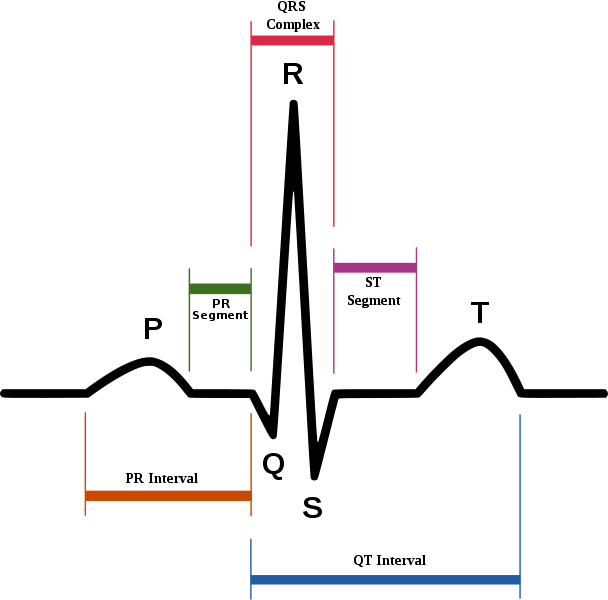
\includegraphics[scale=0.37]{./Abrak/Egyeb/ecg_wiki.png}
   \caption{Az EKG jel egy szívütése, illetve annak főbb diagnosztikai jellemzői.}
		\label{fig:ekg}
\end{center}
\end{figure}
Az EKG jelek méréséhez több elektródát is használhatunk. Így megkülönböztetünk végtagi és mellkasi elvezetéseket. A gyakorlatban a $12$ csatornás EKG jelek a legelterjedtebbek. A mintavételezési frekvencia változó, a dolgozatban $360$ Hz-es jeleket dolgoztunk fel. Ez azt jelenti, hogy egy elvezetésen másodpercenként $360$ adat keletkezik. Így az eljárás során keletkező EKG jelek hatékony tárolása fontos kutatási területnek számít. Az adatok tömörítésére különösen nagy szükség van a 24-órás Holter-felvételeknél, illetve a szűk keresztmetszetű adatátviteli vonalaknál (pl. mobil EKG). 

Az irodalomban ismert tömörítő algoritmusokat \cite{unifiedReview} alapján három kategóriába sorolhatjuk: 1) egyszerű paraméteres becslések (pl.: interpoláció, különbségi kódolás, stb.), 2) direkt módszerek (pl.: csúcsok, meredekségek, stb. tárolása), 3) transzformációs eljárások. Az utóbbi osztály tartalmazza azokat az algoritmusokat, melyek a jelet egy előre adott függvényrendszer szerinti sorfejtéssel approximálják. Így az eredeti adatsorozat helyett csak az együtthatókat és a rendszer paramétereit kell tárolnunk. Ide tartozik a dolgozatban bemutatott algoritmus is. Nevezetesen, az eredeti adatsorozatot Hermite-polinomok segítségével fogjuk közelíti. A módszer alapját képező eljárás \cite{hexp3}, jól ismert az irodalomban, mely nem csak a jelek tömörítéséhez, de azok modellezéséhez \cite{hexp2}, illetve osztályozásához \cite{hexp1, hexp4} is alkalmazható. A dolgozatban az EKG jelekkel való hasonlóságuk miatt Hermite-függvényeket használunk az adatok reprezentálásához. Ezeket egy argumentum transzformáción keresztül szabad paraméterekkel egészítjük ki. Ennek köszönhetően az eredeti jelet egy adaptív bázisban írhatjuk fel. Az említett paraméterek optimális megválasztásához különböző algoritmusokat használtunk, melyek hatékonyságát a tömörítés, pontosság és futásidő szempontjából is megvizsgáltuk. Mivel az EKG jelek diszkrét adatsorozatok, ezért a módszert \cite{hexp5} alapján implementáltuk diszkrét ortogonális Hermite-polinomokra is. A dolgozatban különböző tesztekkel demonstráljuk az algoritmus hatékonyságát. Ehhez, több órányi, zajjal terhelt, valódi EKG felvételt használtunk. Ezen keresztül a bemutatott módszert összehasonlítottuk egy másik, az irodalomban jól ismert tömörítő algoritmussal is \cite{jpeg2000ECG}. 


\chapter{ Approxim\'aci\'o  Hilbert terekben }

\section{Jelek k\"ozel\'\i t\'ese}	
Az EKG jelek feldolgoz\'aval kapcsolatban sz\'amos gyakorlati probl\'ema mer\"ulhet fel. P\'eld\'aul  hosszan tart\'o  m\'er\'esek eset\'en  a be\'erkez\H o jel t\'arol\'as\'ahoz indokolatlanul nagy er\H oforr\'as sz\"uks\'eges, illetve, az EKG esetenk\'ent zajjal terhelt, ami megnehez\'\i ti a k\'es\H obbiekben annak elemz\'es\'et. Mindk\'et probl\'em\'ara egyszerre ad kiel\'eg\'\i t\H o megold\'ast, ha a jeleket  valamely $\mathcal H$ Hilbert-t\'er  sima f\"uggv\'enyeib\H ol \'all\'o $(\Phi_n, n\in\Bbb N)$ ortogon\'alis b\'azis\'aban reprezent\'aljuk \'es v\'eges sok $\Phi_0,\Phi_1,\ldots,\Phi_n$ b\'azisbeli elem line\'aris kombin\'aci\'oj\'aval k\"ozel\'\i tj\"uk. Az $f\in\mathcal H$ jel
legjobb k\"ozel\'\i t\'es\'et a t\'er $\|\cdot\|$ norm\'aj\'aban az
\begin{equation*}
S_nf:=\sum_{k=0}^n\langle f,\Phi_k\rangle \Phi_k
\end{equation*}
projekci\'o szolg\'altatja, ahol $\langle\cdot,\cdot\rangle$ az $\mathcal  H$ t\'er
skal\'aris szorzat\'at jel\"oli. A jel \'es a k\"ozel\'\i t\'es elt\'er\'es\'enek n\'egyzete  a következő alakban írható fel:
\begin{equation*}
\|f-S_nf\|^2=\|f\|^2-\sum_{k=0}^n|\langle f,\Phi_k\rangle|^2 \,.
\end{equation*}
Adott hib\'an bel\"uli k\"ozel\'\i t\'est v\'eve a jel helyett  el\'eg az
$S_nf$ approxim\'aci\'ot reprezent\'al\'o  $\langle f,\Phi_k\rangle\ (k=0,1,\ldots, n)$ Fourier-egy\"utthat\'okat t\'arolni.  Az így kapott approximációval a zaj is kiszűrhető az eredeti jelből.  A k\"ozel\'\i t\'es megval\'os\'\i t\'as\'ahoz a klasszikus ortogon\'alis rendszerek k\"oz\"ul  EKG g\"orb\'ek k\"ozel\'\i t\'es\'ere  az Hermite-f\'ele f\"uggv\'enyek bizonyultak haszn\'alhat\'onak. Ezt t\'amsztja al\'a a \cite{hexp3} dolgozat is. A Hermite-f\"uggv\'enyek alkalmaz\'asa többek között azzal indokolhat\'o, hogy grafikonjuk hasonl\'\i t az EKG g\"orb\'ekre. Ezt a tulajdonságot a \ref{fig:phi0-3} ábra szemlélteti.
%\begin{figure}[H]
%\begin{center}
   %\includegraphics[width=120mm]{H_n.png}
   %\caption{Hermite f\"uggv\'enyrendszer}
%\end{center}
%\end{figure}
\begin{figure}
  \centering
\subfigure[$\Phi_{0}(x)$]{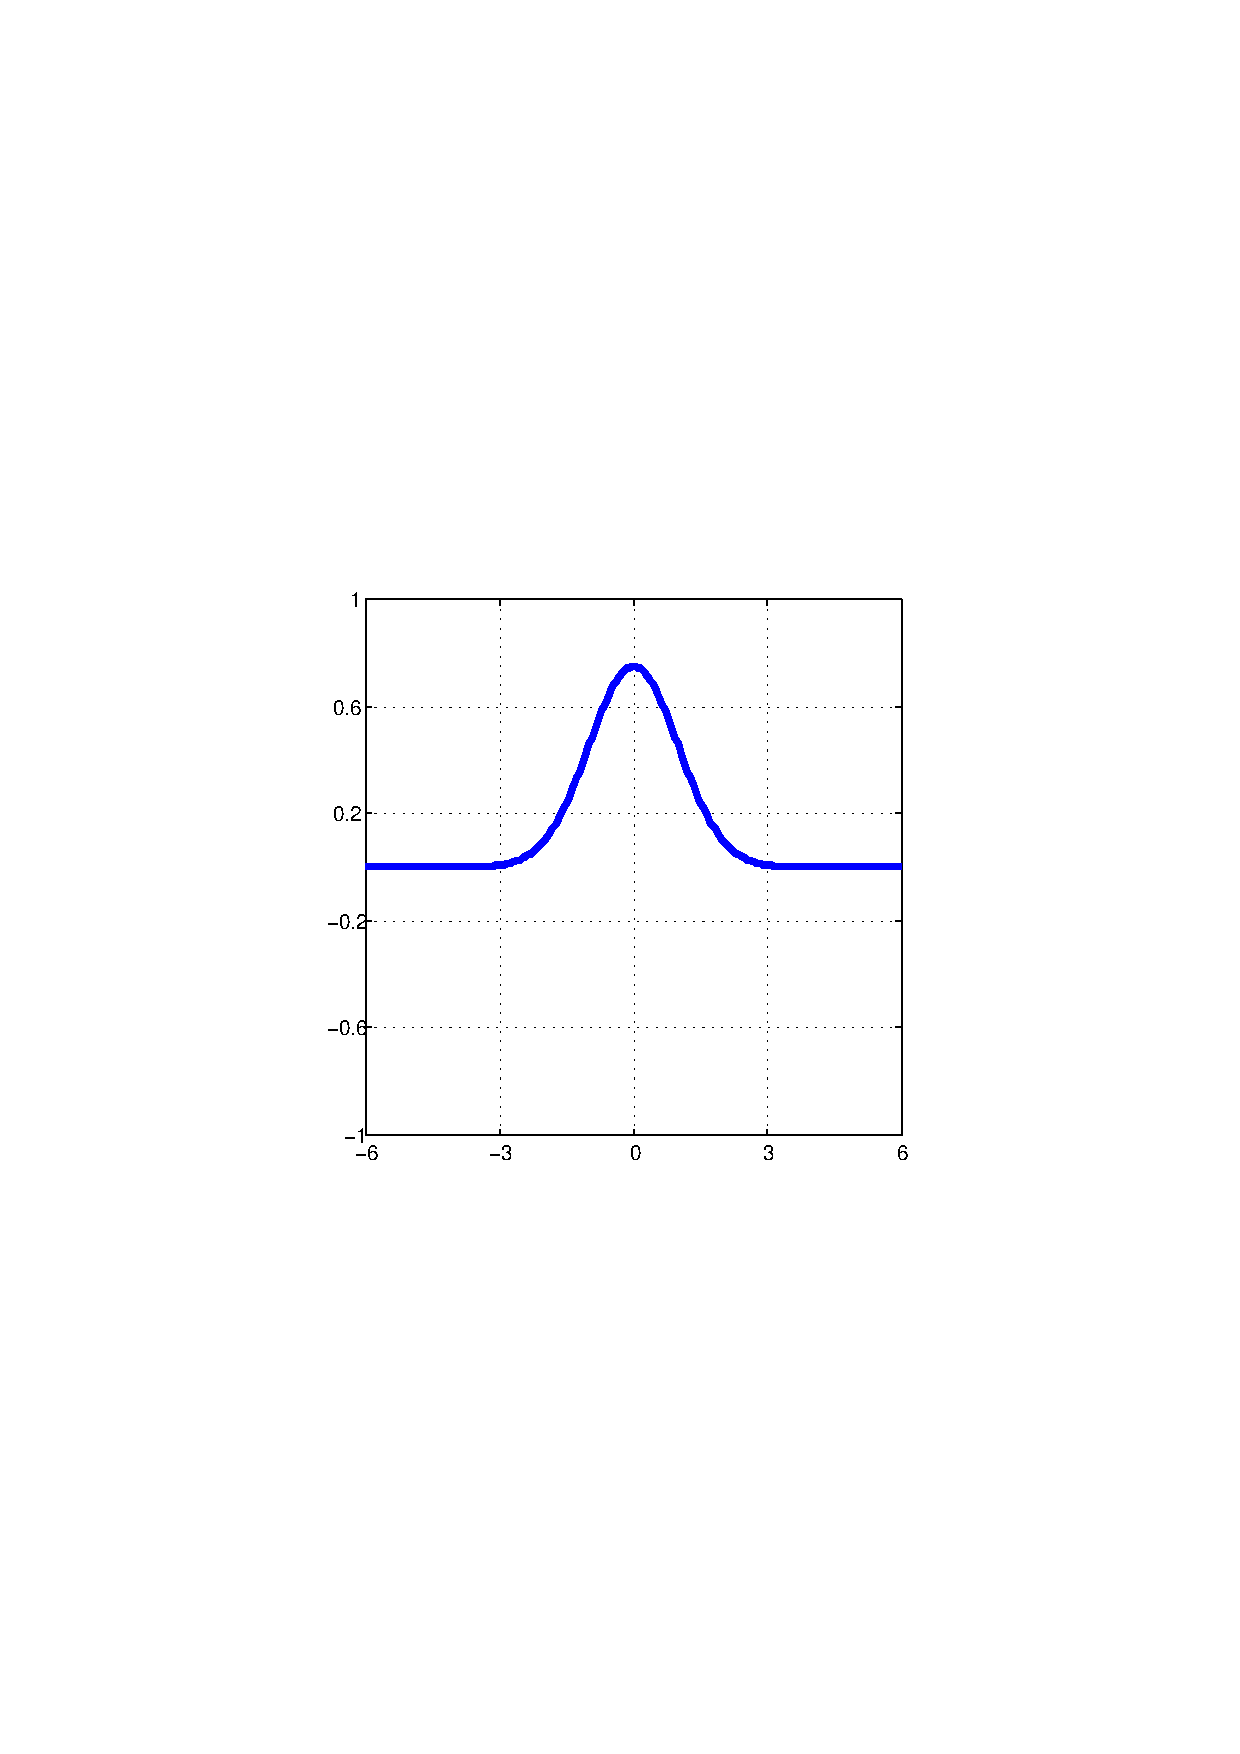
\includegraphics[scale=0.34,trim=150 280 150 280,clip]{./Abrak/Egyeb/phi0.pdf}} 
\subfigure[$\Phi_{1}(x)$]{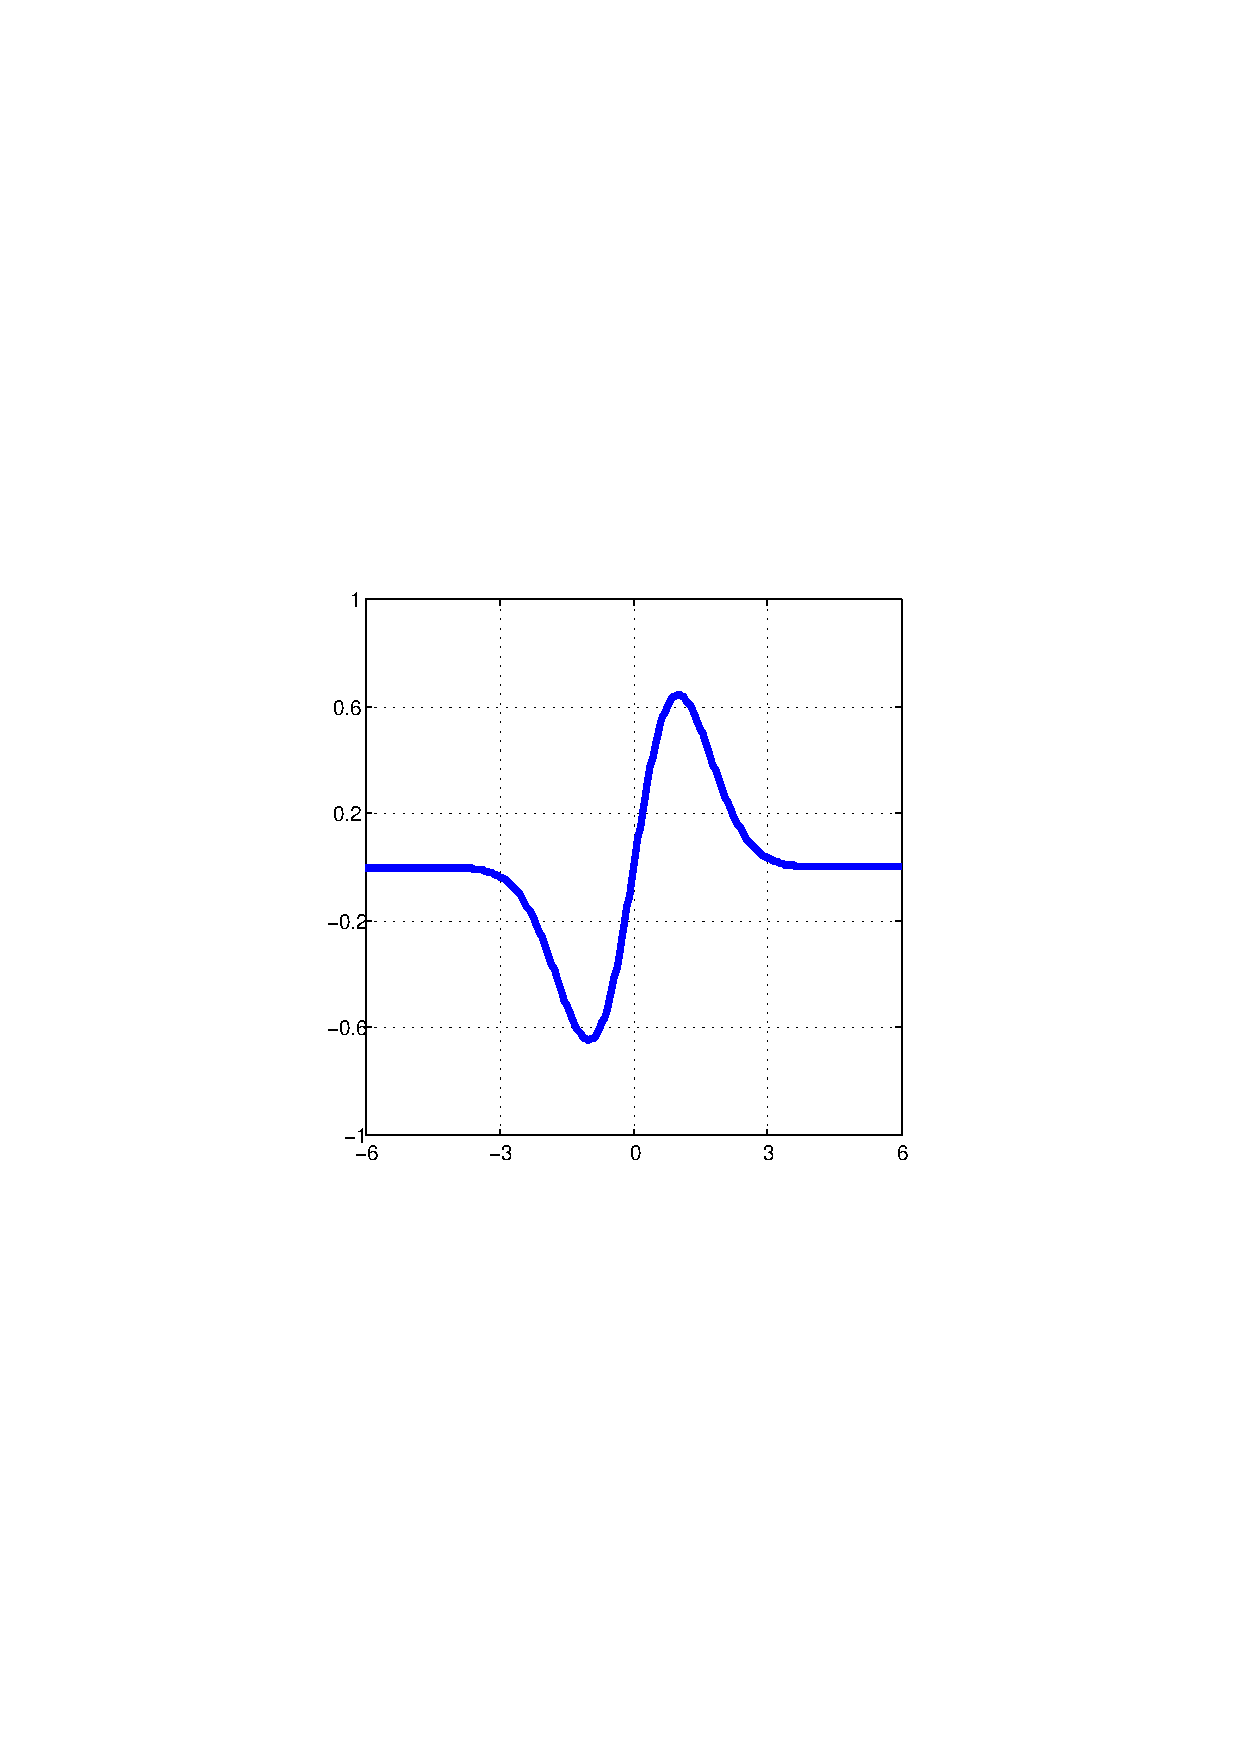
\includegraphics[scale=0.34,trim=150 280 150 280,clip]{./Abrak/Egyeb/phi1.pdf}}
\subfigure[$\Phi_{2}(x)$]{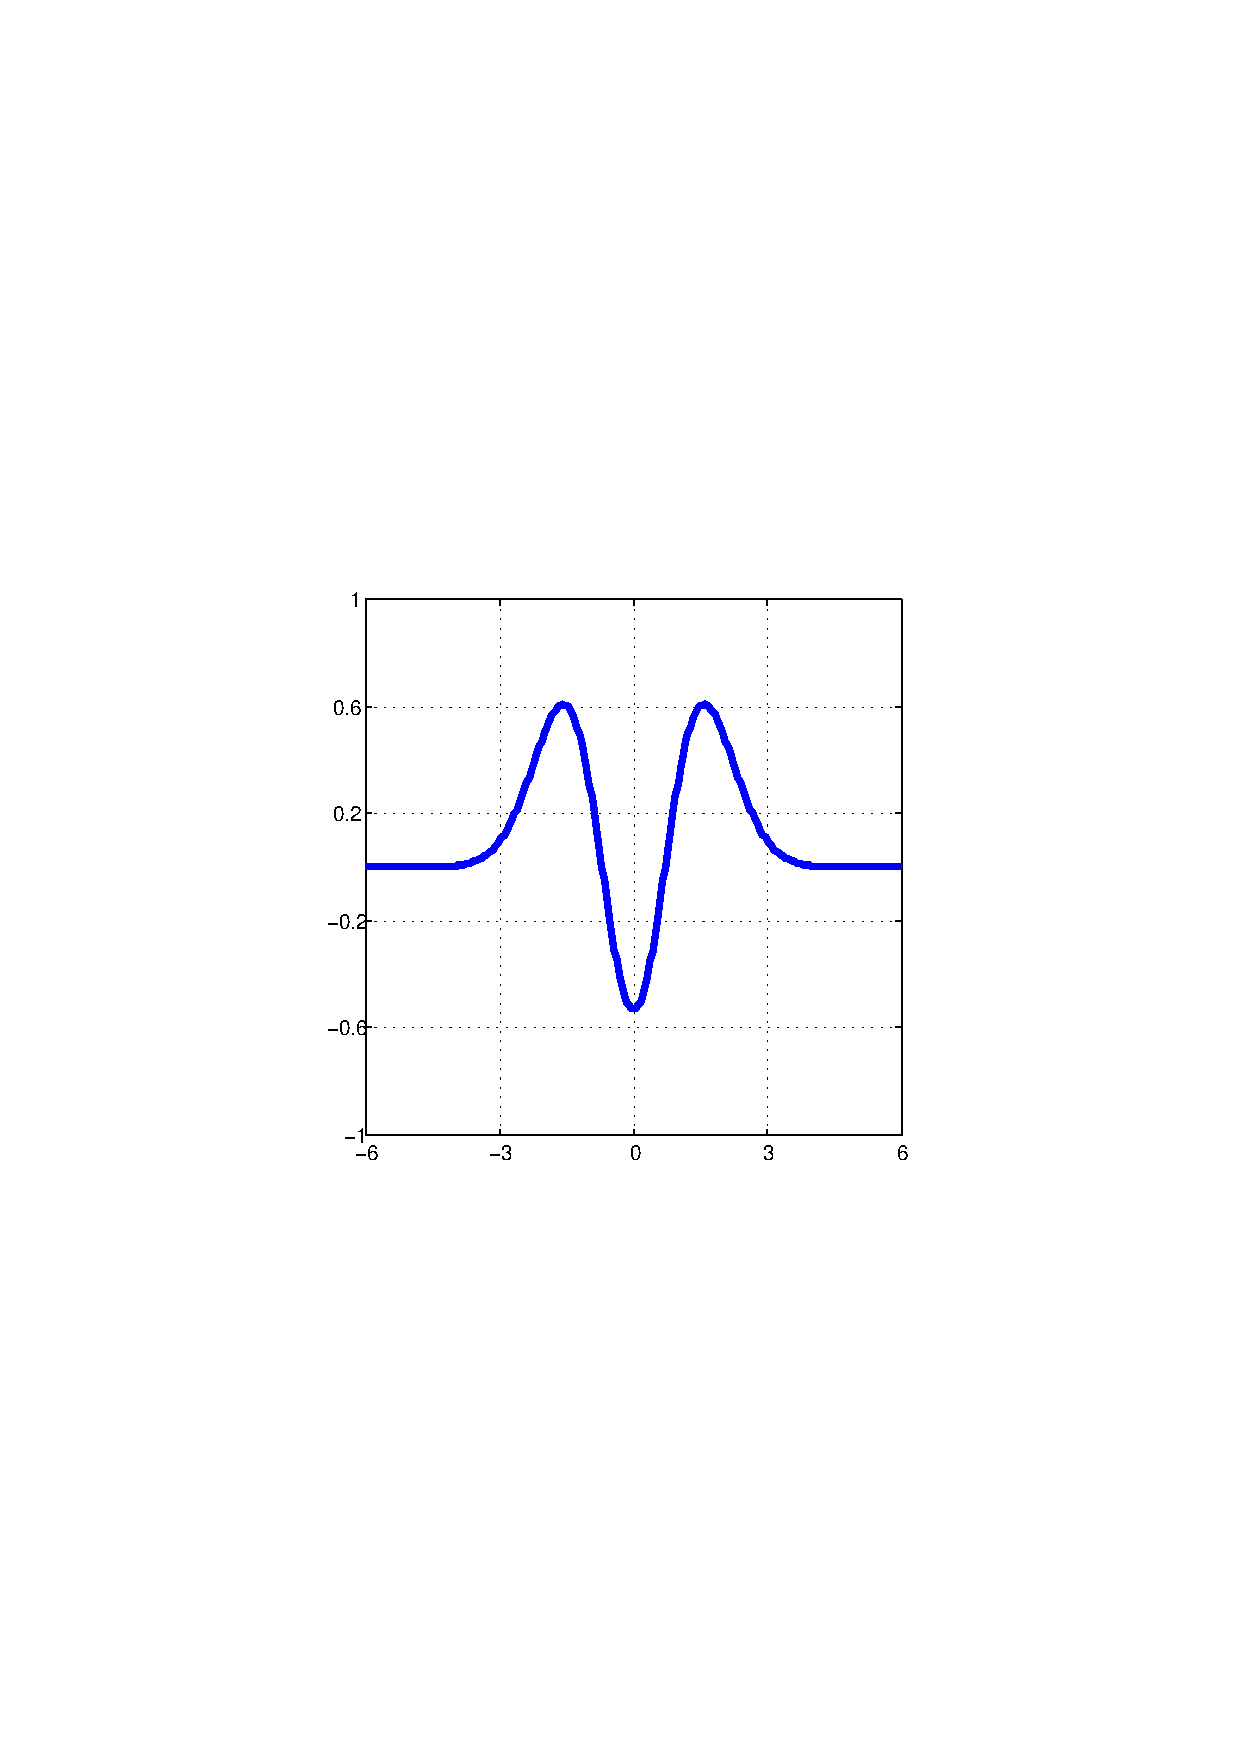
\includegraphics[scale=0.34,trim=150 280 150 280,clip]{./Abrak/Egyeb/phi2.pdf}} 
\subfigure[$\Phi_{3}(x)$]{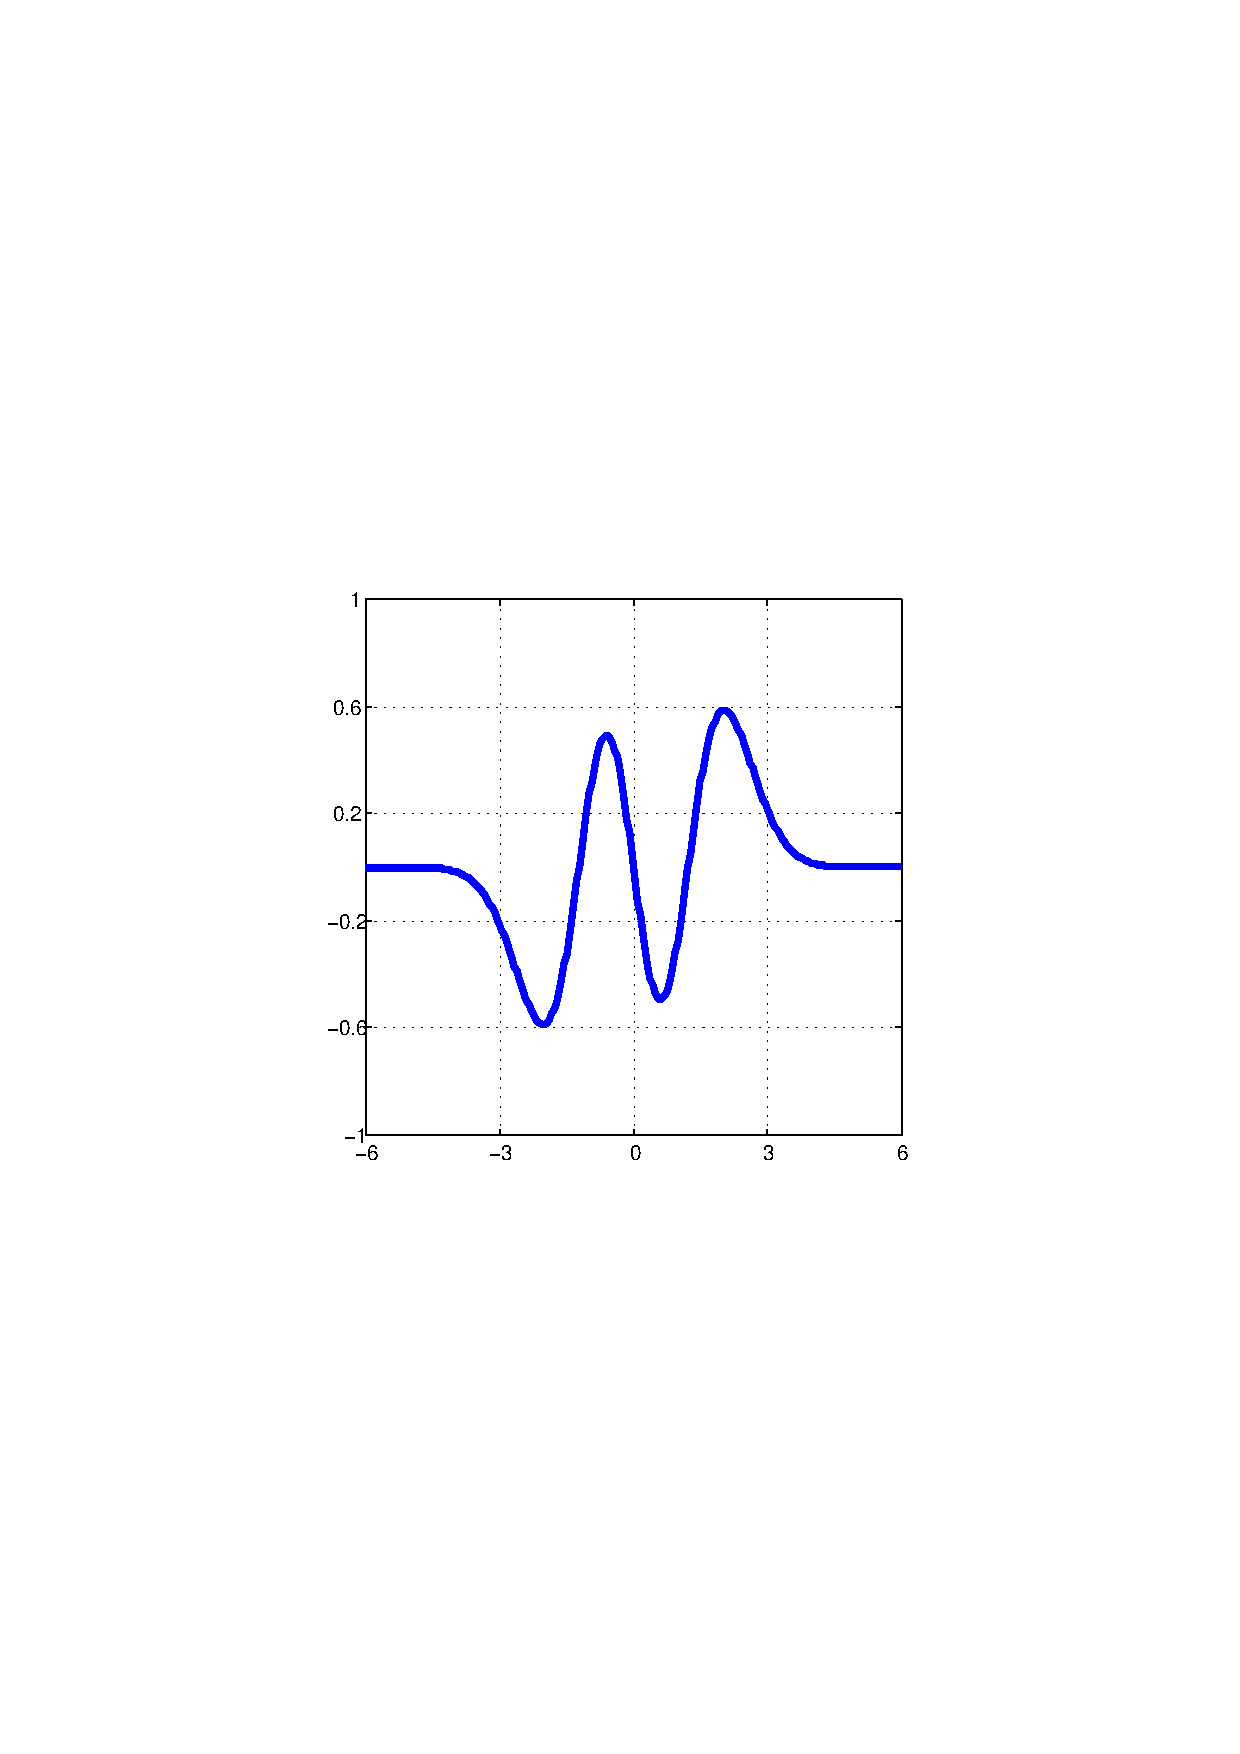
\includegraphics[scale=0.34,trim=150 280 150 280,clip]{./Abrak/Egyeb/phi3.pdf}}
\caption{A Hermite-f\"uggv\'enyrendszer első négy tagja.}
\label{fig:phi0-3}
\end{figure}

A dolgozatban  az $\Bbb R$ sz\'amegyenesen (Lebesgue-mérték szerint) n\'egyzetesen integr\'alhat\'o f\"uggv\'enyek $\mathcal H$ Hilbert-tere helyett elegend\H o a szakaszonk\'ent folytonos, az $\Bbb R$-en  n\'egyzetesen integr\'alhat\'o f\"uggv\'enyek $\mathcal F$ euklideszi ter\'et haszn\'alni. Ebben a t\'erben a skal\'aris szorzat \'es a norma a következő alakban \'\i rhat\'o fel:
\begin{equation}
 \langle f,g\rangle:=\int_{-\infty}^\infty f(t)g(t)\, dt,\ \ \|f\|:=\sqrt{\langle f,f\rangle}\ \ (f,g\in\mathcal F)\,.
\label{eq:dotprod}
\end{equation}
Továbbá, a
 \begin{equation*}
 \Phi_n(x):=H_n(x)e^{-x^2/2}/\sqrt{\pi^{1/2}2^n n!}\quad \ (n\in\Bbb N)
 \end{equation*}
norm\'alt Hermite-f\"uggv\'enyek (teljes) ortonorm\'alt rendszert alkotnak a $\mathcal F$ t\'eren:
  \begin{equation*}
   \langle \Phi_n,\Phi_m\rangle=\delta_{nm}\ \ (m,n\in\Bbb N),\quad
  \|f-S_nf\|\to 0\ (n\to\infty)\,.
   \end{equation*}
Itt $H_n\ (n\in\Bbb N)$ jel\"oli az Hermite-f\'ele polinomokat.

\section{Hermite-f\"uggv\'enyek}

Az Hermite-f\"uggv\'enyek alkalmaz\'as\'anak sz\'amos el\H onye van:

\bigskip
i) A $\Phi_n\ (n\in\Bbb N)$ rendszer z\'art (teljes) az $\mathcal F$ t\'eren.

\bigskip
ii) A $\Phi_n(x)$ f\"uggv\'enyek gyorsan tartanak $0$-hoz, ha $|x|\to \infty$:
$$
|\Phi_n(x)|\le M_n e^{-x^2/4}\le M_n\ \ (x\in\Bbb R, n\in\Bbb N).
$$

\bigskip
iii) A $\Phi_n$ f\"uggv\'enyek (stabil) m\'asodrend\H u rekurzi\'oval sz\'am\'\i that\'ok:
\begin{equation}
\begin{split}
&\Phi_0(x):=e^{-x^2/2}/\pi^{1/4},\ \Phi_1(x):=\sqrt{2}\, x e^{-x^2/2}/\pi^{1/4}\\
&\Phi_n(x)=\sqrt{\frac 2 n} x \Phi_{n-1}(x)-\sqrt{\frac{n-1}n}\Phi_{n-2}(x)\ \ (x\in\Bbb R, n\ge 2)
\end{split}
\end{equation}

\bigskip
iv) A $\Phi_n'$ deriv\'altak kifejezhet\H ok a $\Phi_n, \Phi_{n-1} $ f\"uggv\'enyekkel:
\begin{equation}
\Phi_n'(x)=\sqrt{2n}\Phi_{n-1}(x)-x\Phi_n(x)\ \ (x\in\Bbb R, n\in\Bbb N,\Phi_{-1}=0)
\end{equation}

\section{Rendszerek affin transzform\'altja }

A jelek reprezent\'aci\'oja  f\"ugg az id\H osk\'ala $0$ pontj\'anak \'es az egys\'eg
megv\'alaszt\'as\'at\'ol. Ezeket a param\'etereket  a gyakorlatban \"onk\'enyesen szokták
 beállítani. Példaként említjük a \cite{hexp4, hexp5} cikkeket, melyekben az EKG felvétel minden egyes szívütéséhez ugyanazokat a paramétereket használták. Így általában a közelítés hibája nem optimális, sőt adott esetben az approximáció teljesen rossz eredményt is adhat. Gondoljunk például az átlagtól eltérő, abnormális szívütésekre. Ezzel \"osszef\"ugg\'eben felvethet\H o a k\'erd\'es, hogyan lehet optim\'alisan megv\'alaszthatani a rendszer paramétereit.
Az  approxim\'aci\'o pontoss\'ag\'at jav\'\i thatjuk azonos egy\"utthat\'o sz\'am mellett, amennyiben az  Hermite-f\"uggv\'enyek helyett azok
\begin{equation}
\Phi_n^{a,\lambda}(x):=\Phi_n(\lambda x+a)\ \  (x,a\in\Bbb R, \lambda>0)
\end{equation}
affin transzform\'altjait haszn\'aljuk. A $\sqrt{\lambda}\Phi_n^{a,\lambda}\ (n\in\Bbb N)$ rendszer is ortonorm\'alt \'es teljes az $\mathcal F$ t\'eren. Ebben az esetben
az $f$ legjobb approxim\'aci\'oja az
\begin{equation}
S_n^{a,\lambda}f:=\sum_{k=0}^n\langle f,\Phi_k^{a,\lambda}\rangle\Phi_k^{a,\lambda}\ \
(n\in\Bbb N, a\in\Bbb R,\lambda>0)
\label{eq:hilaprx}
\end{equation}
projekci\'o \'es a k\"ozel\'\i t\'es hib\'aja az $a$ transzl\'aci\'os \'es a $\lambda$ dilat\'aci\'os param\'eter f\"uggv\'enye:
\begin{equation*}
D^2_n(a,\lambda):=\|f\|^2-\sum_{k=0}^n|\langle f,\Phi_k^{a,\lambda}\rangle|^2\,.
\end{equation*}
E k\'et szabad param\'eter optimaliz\'al\'as\'aval azonos egy\"utthat\'osz\'am mellett, az eredeti Hermite-polinomokkal t\"ort\'an\H o  approxim\'aci\'ohoz k\'epest pontosabb k\"ozel\'\i t\'est \'erhet\"unk el. A $D_n$ f\"uggv\'eny minimaliz\'al\'asa ekvivalens  az
\begin{equation}
 F_n(a,\lambda):=\sum_{k=0}^n|\langle f,\Phi_k^{a,\lambda}\rangle|^2
\label{eq:Fnfuggv}
\end{equation}
 f\"uggv\'eny maximum\'anak meghat\'aroz\'as\'aval. Továbbá, a param\'eteres integr\'alok tulajdons\'agaib\'ol k\"ovetkezik, hogy az
\begin{equation*}
 A_n(a,\lambda):=\langle f,\Phi_k^{a,\lambda}\rangle \quad  ((a,\lambda)\in T:=\Bbb R\times (0,\infty))
\end{equation*}
 Fourier-egy\"utthat\'ok a $T$ tartom\'anyon a param\'eterek sima f\"uggv\'enyei. Bebizony\'\i that\'o, hogy $\lambda\to 0$ \'es $|a|+\lambda\to \infty$ eset\'en
 $F_k(a,\lambda)\to 0$, k\"ovetkez\'esk\'eppen az $F_n$ f\"uggv\'enynek l\'etezik a
 maximuma \'es a $D_n$ f\"uggv\'enynek l\'etezik a minimuma. A bizonyítás részleteit az \ref{app:aprx} F\"uggel\'ek tartalmazza. 

A \ref{fig:hibafuggveny1} ábra az $F_n(a,\lambda)$ f\"uggv\'enyt szeml\'elteti f\'enyintenzit\'as \'es perspektivikus \'abr\'azol\'ast haszn\'alva. A fehér vonal a lokális szélsőértékek helyét, a pont pedig a globális maximumot jelöli. Előbbi jól láthatóan az $F_n(a,\lambda)$ függvényen egy ún. hegygerincet képez. Ezt szemlélteti \ref{fig:hibafuggveny2} ábra is, melyen a jel k\"ozel\'\i t\'esét is kirajzoltuk a globális maximum helynek megfelel\H oen.
%\begin{figure}[htb!]
%\begin{center}
   %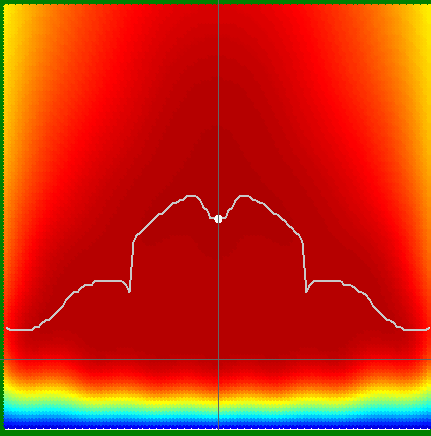
\includegraphics[scale=0.39]{./Abrak/Ereszkedo/F_2sz.png}
  %\caption{Az $F_n$ sz\'\i nk\'odos \'abr\'azol\'asa.}
	%\label{fig:hibafuggveny1}
%\end{center}
%\end{figure}
\begin{figure}[htb!]
  \centering
\subfigure[Hibafüggvény 2D.]{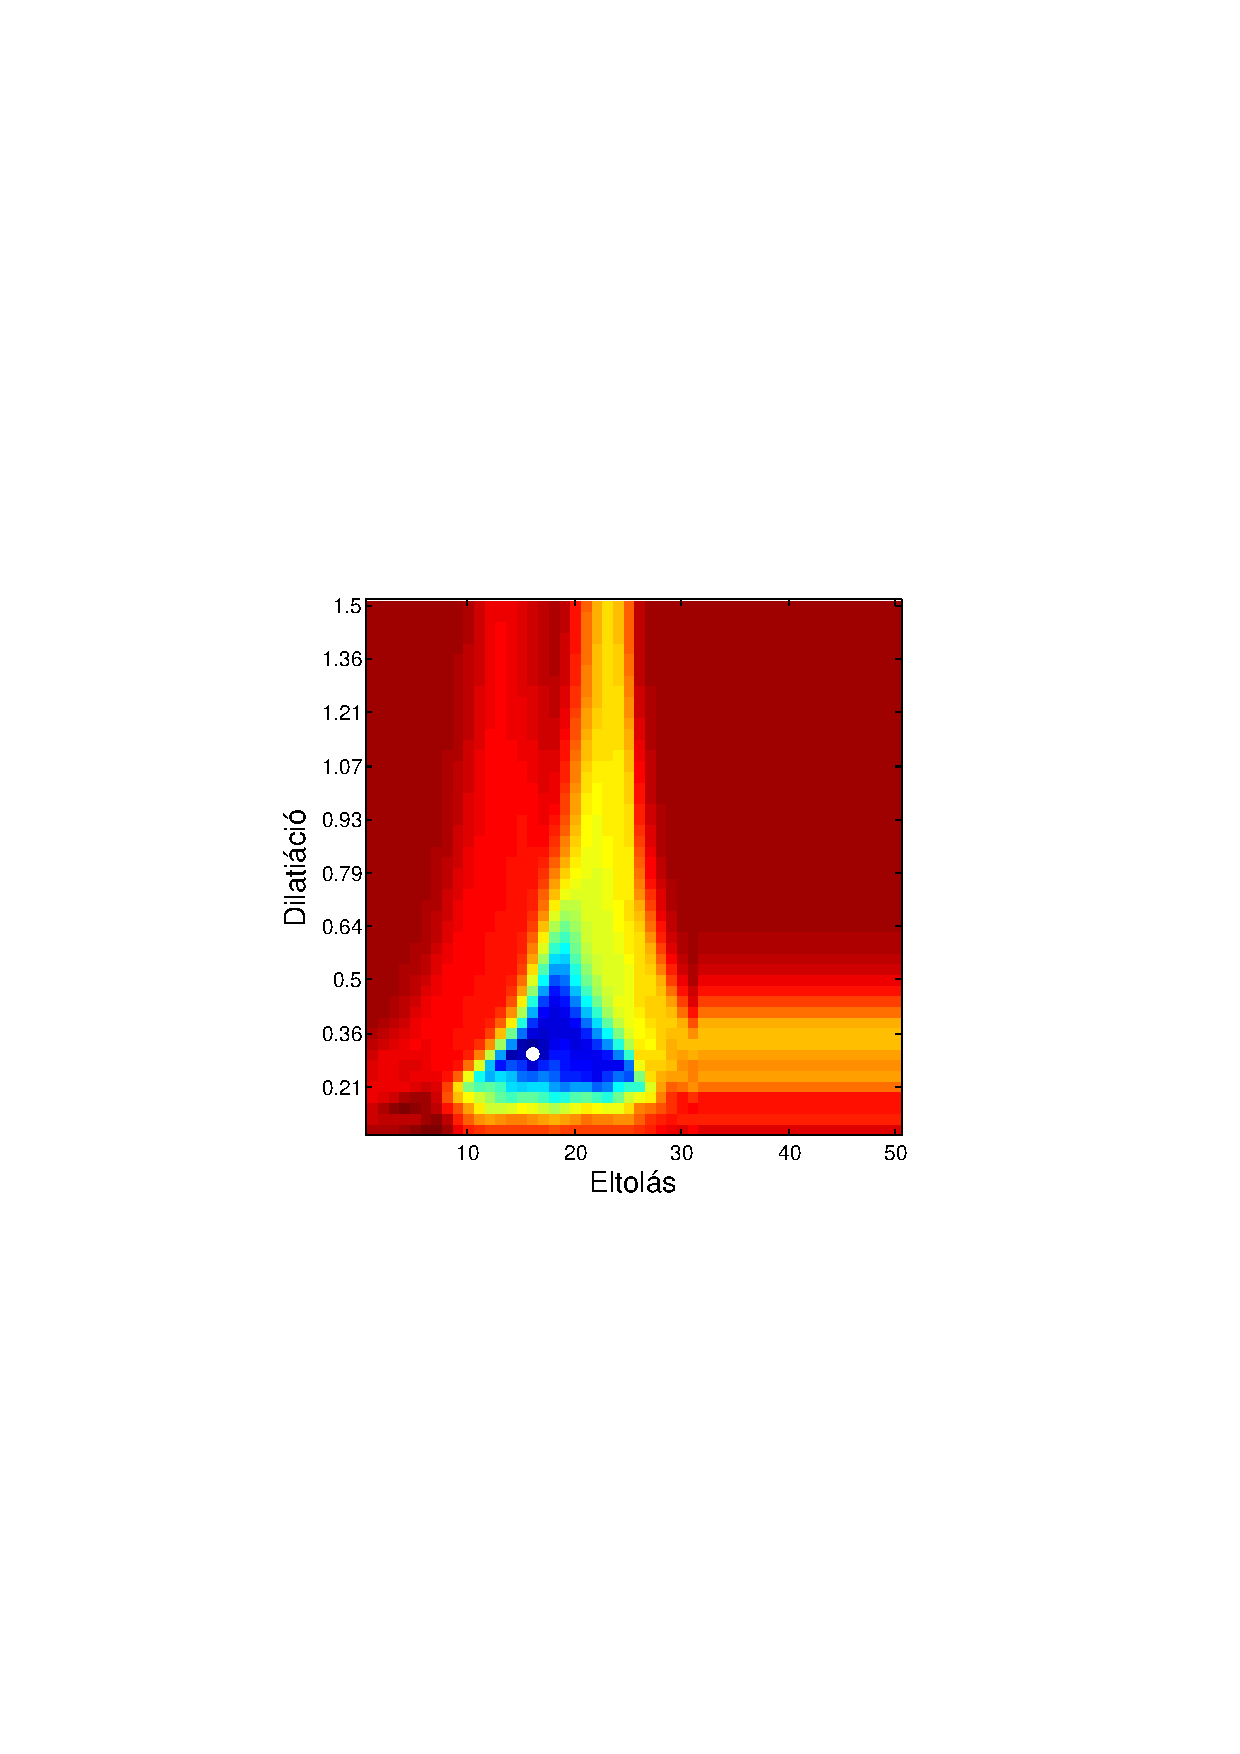
\includegraphics[scale=0.35,trim=130 260 140 280,clip]{./Abrak/Ereszkedo/TDKabra1_felul.pdf}} 
\subfigure[Hibafüggvény 3D.]{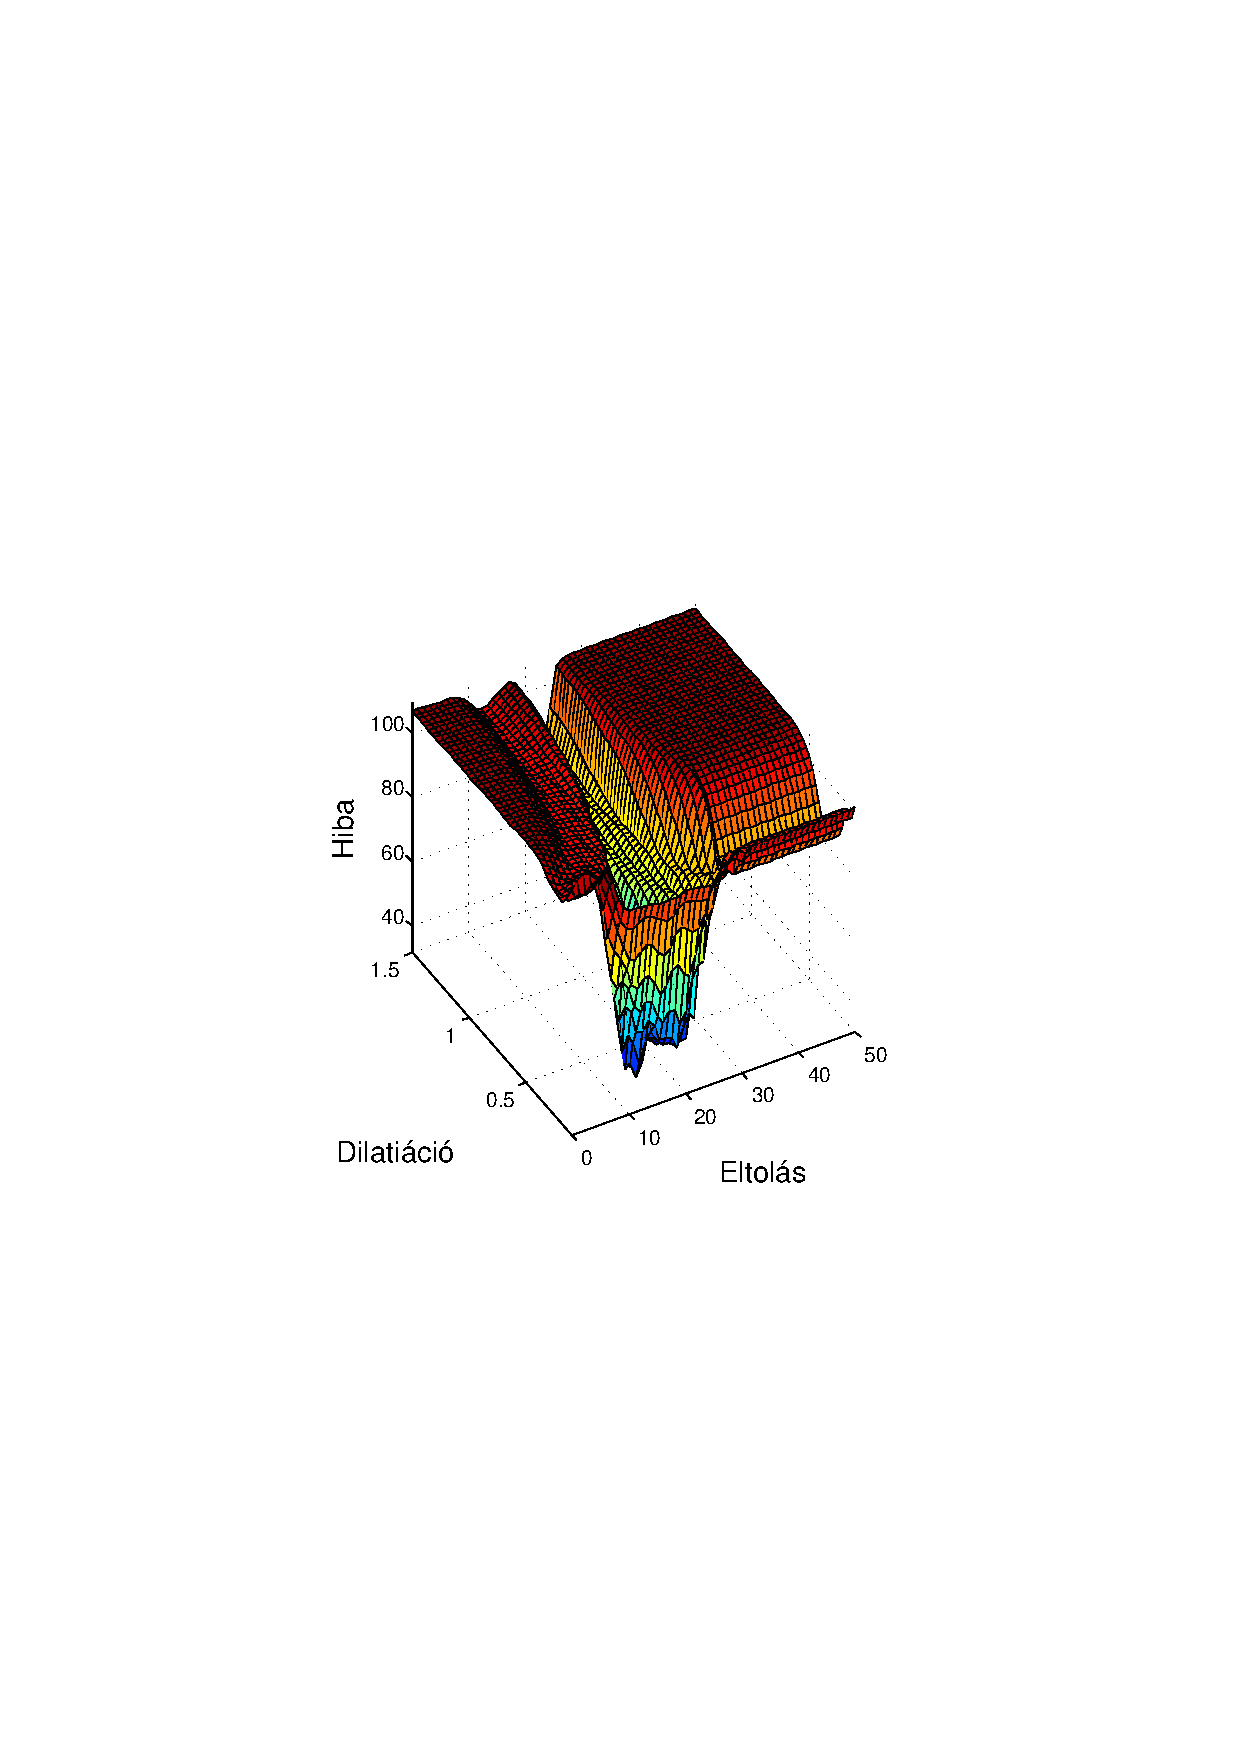
\includegraphics[scale=0.4,trim=160 270 140 280,clip]{./Abrak/Ereszkedo/TDKabra1_oldal}} 
\subfigure[QRS komplexus.]{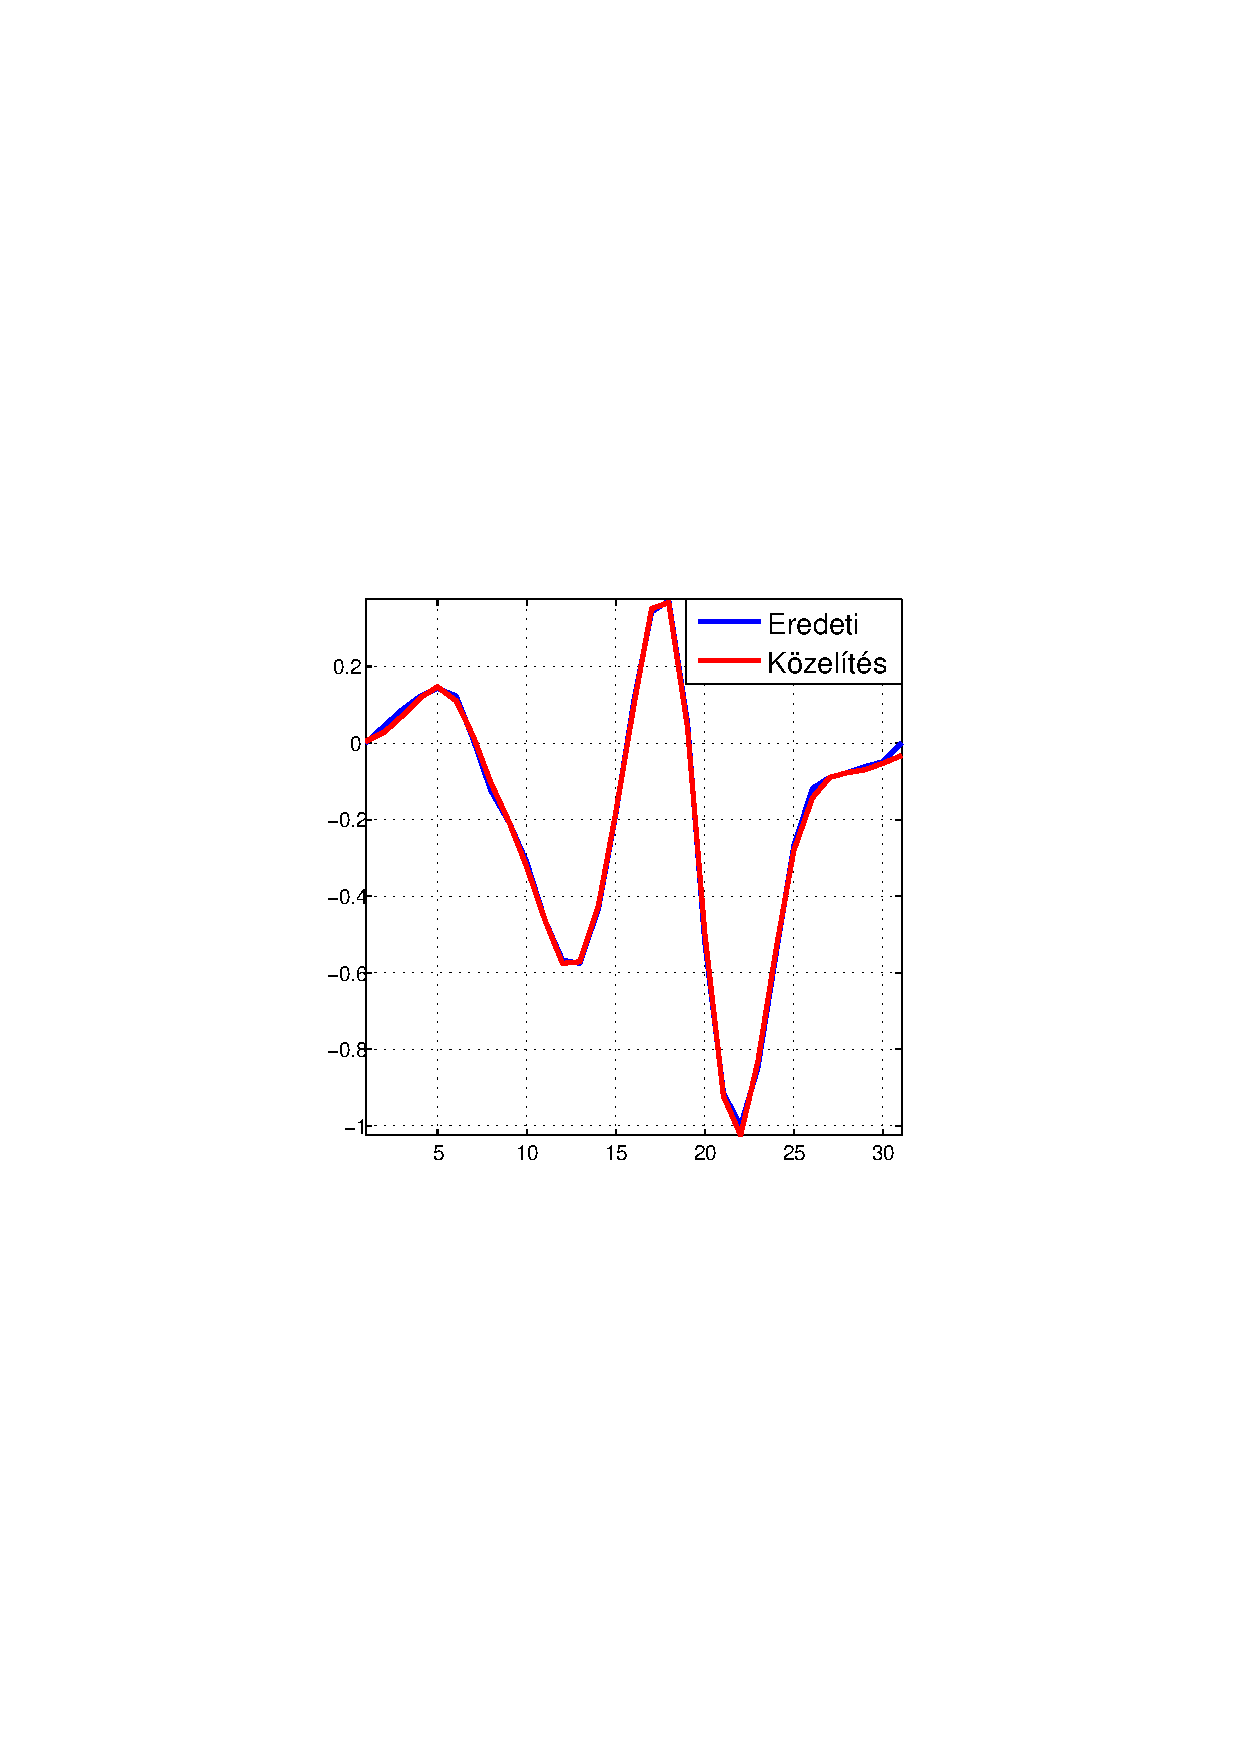
\includegraphics[scale=0.35,trim=160 260 140 280,clip]{./Abrak/Ereszkedo/TDKabra1.pdf}}
\caption{A $D_n$ \'altal meghat\'arozott fel\"ulet, \'es approxim\'aci\'o.}
\label{fig:hibafuggveny1}
\end{figure}
\begin{figure}[htb!]
  \centering
\includegraphics[scale=0.225]{./Abrak/Ereszkedo/er36_a.PNG}
\hspace{10mm}
\includegraphics[scale=0.225]{./Abrak/Ereszkedo/er36_b.PNG}
\caption{Az $F_n$ \'altal meghat\'arozott fel\"ulet, \'es approxim\'aci\'o.}
\label{fig:hibafuggveny2}
\end{figure}

\chapter{ Optimaliz\'al\'o  algoritmusok}

 A dolgozatban h\'arom algoritmust alkalmaztunk az $F_n(a,\lambda)$ függvény maximumának meghatározásához. A módszerek kiválasztásánál figyelembe vettük az alkalmazási területek gyakoriságát, az eljárások típusát, és gyorsaságát. Ezért implementáltunk egy determinisztikus szimplex algoritmust \cite{NelderMeadSimplex}, egy raj alapú nem determinisztikus optimalizációt \cite{basic_pso} és a gradiens módszert \cite{numopt}. Felhívjuk a figyelmet arra, hogy az első két esetben csak a hibafüggvény értékeire támaszkodunk. Ezzel ellentétben, a gradiens módszer konstrukciójához szükség van az $F_n(a,\lambda)$ függvény parciális deriváltjaira is. Megjegyezzük, hogy ennek levezetése nem triviális, ezért a dolgozat eredményinek szerves részét képezi.     

\section{Leggyorsabb ereszked\'es m\'odszere}

A leggyorsabb ereszked\'es  m\'odszere (m\'as sz\'oval a gradiens m\'odszer) alkalmas arra, hogy egy $f:\Bbb R^n\to\Bbb R$ t\"obbv\'altoz\'os  f\"uggv\'eny   minimum\'at (maximum\'at)
  meghat\'arozzuk. A m\'odszer l\'enyege, hogy egy $x_0\in\Bbb R^n$ kezd\H opont\'ol
kiindulva  a
\begin{equation*}
f'(x_0)=\grad\, f(x_0)=(\partial_1 f(x_0),\cdots,\partial_n f(x_0))\in\Bbb R^n
\end{equation*}
 deriv\'altat (gradienst) felhasználva a f\"uggv\'enyt lesz\H uk\'\i tj\"uk az $x_0$ ponton \'athalad\'o, gradiens ir\'any\'u $x_0+tf'(x_0)\ (t\in \Bbb R)$ egyenesre. Az így kapott
$ F_0(t):=f(x_0+tf'(x_0))\ (t\in\Bbb R)$ egyv\'altoz\'os f\"uggv\'enynek meghat\'arozzuk  a
$t_0$ minimum hely\'et: $F_0(t_0)=\min_{t\in\Bbb R}F_0(t)$, majd az elj\'ar\'ast az $x_1:=x_0+t_0f'(x_0)$ pontban folytatjuk.  Tehát az $x_k\in \Bbb R^n$ ismeret\'eben \'ertelmezz\"uk az $F_k(t):=f(x_k+tf'(x_k))\ (t\in\Bbb R)$  f\"uggv\'enyt,  legyen
 $t_k$ ennek a minimun helye \'es
\begin{equation*}
x_{k+1}:=x_k+t_kf'(x_k),\ \ \text{ahol}\ \ \ F_k(t_k)=\min_{t\in\Bbb R} F_k(t).
\end{equation*}
Sz\'amos olyan f\"uggv\'enyoszt\'aly ismert, amelyek minimum helyének meghatározásához alkalmazhat\'o a leggyorsabb ereszked\'es elve. Ilyen p\'el\'aul $\Bbb R^n$-ben a
pozit\'\i v definit kvadratikus alakok oszt\'alya. Jel\"olje $\langle\cdot,\cdot\rangle $
az $\Bbb R^n$ skal\'aris szorzat\'at, legyen  $A\in\Bbb R^{n\times n}$
egy pozit\'\i v definit m\'atrix \'es $b\in\Bbb R^n.$ Ekkor az
\begin{equation*}
 f(x):=\langle Ax-b, x\rangle \quad (x\in\Bbb R^n)
\end{equation*}
 f\"uggv\'enynek van minimuma \'es ebben az esetben az $x_k\ (k\in\Bbb N)$ sorozat az $f$ f\"uggv\'eny $x^\ast$ minimum hely\'ehez  konverg\'al. Mivel a minimum helyre $Ax^\ast=b$
 teljes\"ul, ez\'ert a m\'odszer lin\'aris egyenletrendszer megold\'as\'ara is haszn\'alhat\'o. 
\begin{figure}[htb!]
\begin{center}
   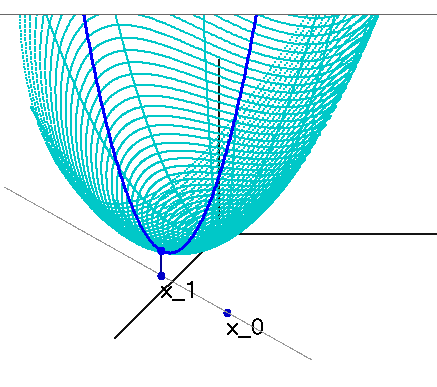
\includegraphics[scale=0.5]{./Abrak/Ereszkedo/Parabola.png}
  \caption{A leggyorsabb ereszked\'es m\'odszere}
\end{center}
\end{figure}

Az $F_n(a,\lambda) \, ((a,\lambda)\in T=\Bbb R\times (0,\infty))$ f\"uggv\'eny maximum\'anak  meghat\'aroz\'as\'an\'al c\'elszerű figyelembe venni, hogy a f\"uggv\'enyt \'abr\'azol\'o fel\"ulet olyan hegyre hasonl\'\i t, amelynek a gerinc magass\'aga csak kiss\'e v\'altozik. A \ref{fig:ersz1}-\ref{fig:ersz2} \'abr\'akon azt szeml\'eltet\-j\"uk, hogy a gradiens m\'odszer ebben az esetben hogyan alkalmazhat\'o. A gradiens vektor zárt alakjának levezetését az \ref{app:aprx} Függelék tartalmazza.

Megjegyezzük, hogy a gradiens módszer egy determinisztikus algoritmus. Ez azt jelenti, hogy azonos inicializálási feltételek mellett, az eljárás ugyanabban a pontban terminál. A konvergencia adott esetben nagyon gyors is lehet, de ez a kezdőponttól függ. Rossz inicializálási feltételek mellett a módszer könnyen elakadhat a hibafüggvény lokális minimumaiban (lsd. Rosenbrock függvény). Ennek elkerülésére a következő fejeztben egy nem determinisztikus raj alapú optimalizáló algoritmust is kirpóbáltunk.

\begin{figure}[h]
  \centering
\subfigure[Ereszkedés lépései.]{\includegraphics[scale=0.27]{./Abrak/Ereszkedo/ERSZ46_a.PNG}} 
\subfigure[Lokális maximumok.]{\includegraphics[scale=0.27]{./Abrak/Ereszkedo/ERSZ46_b.PNG}} 
\subfigure[Maximum környezete.]{\includegraphics[scale=0.27]{./Abrak/Ereszkedo/ERSZ46_c.PNG}}
\caption{$F_n$, leggyorsabb ereszked\'es szimmetrikus jel eset\'en.}
\label{fig:ersz1}
\end{figure}

\begin{figure}[h]
  \centering
\subfigure[Ereszkedés lépései.]{\includegraphics[scale=0.27]{./Abrak/Ereszkedo/ERSZ56_a.PNG}} 
\subfigure[Lokális maximumok.]{\includegraphics[scale=0.27]{./Abrak/Ereszkedo/ERSZ56_b.PNG}} 
\subfigure[Maximum környezete.]{\includegraphics[scale=0.27]{./Abrak/Ereszkedo/ERSZ56_c.PNG}}
\caption{$F_n$, leggyorsabb ereszked\'es asszimmetrikus jel eset\'en.}
\label{fig:ersz2}
\end{figure}


\section{Particle Swarm Optimization}
Egy másik lehets\'eges m\'odja a dilat\'aci\'os, illetve transzl\'aci\'os param\'eterek optimaliz\'al\'as\'anak a $Particle$ $Swarm$ $Optimization$ $(PSO)$ algoritmus alkalmaz\'asa. A módszer egy-egy Hermite-f\"uggv\'enyekb\H ol \'all\'o rendszert \'ugynevezett r\'eszecskek\'ent kezel, a keres\'esi teret pedig a hibaf\"uggv\'eny \'ertelmez\'esi tartom\'anya alkotja $( 0 \le \lambda, t\in \Bbb R)$. Az algoritmus
m\H uk\"od\'es\'enek szempontj\'ab\'ol kritikus szerephez jut a r\'eszecsk\'ek dilat\'aci\'os \'es transzl\'aci\'os param\'etereinek megfelel\H o  inicializ\'al\'asa. Mivel a gyakorlati tapasztalatok az EKG jelek esetében azt mutatták, hogy $\lambda$ egy nem túl nagy pozitív valós szám, ezért a dilat\'aci\'os param\'etert minden r\'eszecsk\'ehez $0$ \'es $10$ k\"oz\"ott  hat\'arozzuk meg. A
transzl\'aci\'os param\'etert pedig a jel maximum hely\'enek egy lokális k\"ornyezet\'eben v\'alasztjuk v\'eletlenszer\H uen. Így például a P, QRS, T hullámok maximum helyei jó kezdőpozíciónak bizonyultak. \par
Minden l\'ep\'esben kisz\'am\'\i tjuk az \"osszes
r\'eszecsk\'ere vonatkoz\'oan, hogy az \'altaluk el\H o\'all\'\i tott approxim\'aci\'o mennyire t\'er el az
eredeti jelt\H ol. Az eljárás során minden részecskéhez nyilvántartjuk az eddigi legjobb pozíciót, illetve a teljes raj globális optimumát. Ezeket rendre a $pbest$ és a $gbest$ változókban tároljuk. Az aktuális pozícióban kapott eltérést összehasonlítjuk az eddig megtalált lokális és globális hibákkal. Végül a $pbest,\, gbest$ változókat ennek megfelelően frissítjük.

Az r\'eszecsk\'ehez egy aktu\'alis sebességet is tárolunk. Ez a sz\'am hat\'arozza meg, hogy az egyes
l\'ep\'esekben milyen m\'ert\'ekben v\'altoztatjuk meg a r\'eszecs\-k\'ehez tartoz\'o dilat\'aci\'os
illetve transzl\'aci\'os param\'etereket. A pozíciókhoz hasonlóan a r\'eszecske aktu\'alis
sebességét is friss\'\i teni kell minden lépésben. Ez a k\"ovetkez\H o \"osszef\"ugg\'es alapj\'an
t\"ort\'enik:
\begin{equation*}
v = v + c_1 \cdot rand() \cdot (pbest - presentpos) + c_2 \cdot rand() \cdot (gbest - presentpos),
\end{equation*}
ahol $v$ a r\'eszecske aktu\'alis gyorsul\'asa. Az egyenletben a $c_1$ \'es $c_2$ tanul\'asi param\'eterek seg\'\i ts\'eg\'evel s\'ulyozhat\'o, hogy a r\'eszecsk\'ek sebességét az eddig megtalált lokális vagy globális optimum befolyásolja. Megjegyezzük, hogy tesztek során, minden iterációban az EKG jelek egy konkrét hullámát közelítettük. A részecskék kezdeti transzlációját is ennek megfelelően a P, QRS, T hullámok maximumával inicializáltuk. Annak érdekében, hogy a raj ne "vándorolhasson" el egy másik hullám felé, a $gbest$ pozíció befolyását a kétszeresére növeltük ($c_1=1,\, c_2=2$).  

Mivel a r\'eszecsk\'ek poz\'\i ci\'oja minden lépésben változik, ezért biztosítani kell, hogy a paraméterek konzisztensek maradjanak. Így például gondoskodni kell arról, hogy a $\lambda$ dilatáció  pozitív maradjon, az $a$ transzláció pedig ne legyen nagyobb mint a jel mintaelemszáma.
Az elj\'ar\'as addig folytat\'odik am\'eg kiel\'eg\'\i t\H o eredm\'enyhez nem jutunk
(vagy el nem \'erj\"uk a maxim\'alis l\'ep\'essz\'amot). A $PSO$ algoritmus pszeudok\'odja 
megtal\'alhat\'o a \ref{chp:alg} F\"uggel\'ekben. 

Megjegyezzük, hogy a $PSO$ több szempontból is különbözik a gradiens módszertől. Egyrészt a részecskék pozíciója függ a véletlentől, így azonos inicializálási feltételek mellett sem garantált, hogy ugyanabban a pontban terminál a program. Ezzel és a raj egyedszámának növelésével csökkenthető a lokális optimumban való elakadás lehetősége. Azonban a több részecske, több függvénykiértékelést is jelent, így a futásidő jelentősen megnőhet. A $Nelder-Mead$ módszer egy köztes megoldást jelenthet a futásidő és a lokális optimumban való elakadás kiküszöböléséhez.   

\section{Nelder--Mead szimplex algoritmus}

A $Nelder-Mead$ szimplex algoritmust \cite{NelderMeadSimplex} eredetileg 1965-ben
fejlesztett\'ek ki azzal c\'ellal, hogy l\'etrehozzanak egy elj\'ar\'ast, amely
k\'epes meghat\'arozni egy $f : \Bbb R^n \to \Bbb R$ nemline\'aris f\"uggv\'eny minimum (maximum) hely\'et a  gradiens felhaszn\'al\'sa  n\'elk\"ul, puszt\'an a f\"uggv\'eny\'ert\'ekekre  t\'amszkodva.
Mivel az algoritmust k\'etv\'altoz\'os f\"uggv\'enyekre alkalmazzuk, ez\'ert ebben a speci\'alis esetben szeml\'eltetj\"uk, megjegyezve, hogy hasonl\'o elvek szerint
 m\H uk\"odik az \'altal\'anos $n$ dimenziós eset is. A minimum meghat\'aroz\'a\-s\'ahoz az $f(x_1), f(x_2), f(x_3)$  függvényértékekből indulunk ki, melyek közül egyet lecserélünk az adott lépésben. Nevezetesen, 
\begin{equation*}
f(x_3)\le f(x_2)\le f(x_1)
\end{equation*}
 eset\'en olyan $x'$ helyet keres\"unk, amelyre $f(x')\le  f(x_3)\le f(x_2)$ teljes\"ul \'es az $x_3, x_2, x_1$ ponth\'armasr\'ol az $x_1$-et elhagyva \'att\'er\"unk az $x',x_3, x_2$ h\'armasra. Az $x'$ pontot az el\H oz\H oekb\H ol geometriai transzform\'aci\'okkal sz\'armaztatjuk, felhaszn\'alva az  $x_2x_3$ szakasz $x=(x_2+x_3)/2$ felez\'espontj\'at: 
\begin{equation*}
x'=x_1+\alpha (x-x_1) \quad (\alpha\in\Bbb R)\,.
\end{equation*}
 Az al\'abbi \'abr\'akon szeml\'eltetj\"uk az algoritmusban  haszn\'alt transzform\'aci\'okat. Vegyük észre, hogy $\alpha=2$ esetén $x'$ éppen az $x_1$ pont $x$-re vonatkozó középpontos tükrözése $(T_1).$ Továbbá $\alpha>2$ az eredeti háromszög t\"ukr\"oz\'ese + ny\'ujt\'asa $(T_2),$ az $1<\alpha<2$ pedig t\"ukr\"oz\'eses + zsugor\'\i t\'asnak felel meg $(T_3).$ A $-1<\alpha<0$ param\'eterrel egyszerű zsugor\'\i t\'ast kapunk. V\'eg\"ul az 5. transzform\'aci\'o $(T_5)$ az $x_3$ pontb\'ol t\"ort\'en\H o
 kicsiny\'\i t\'esnek feleltethető meg. Az $x_1$ k\'ep\'et ezekben a transzform\'aci\'okban \'es a hozzá tartoz\'o f\"uggv\'eny\'ert\'ekeket a következő alakban adjuk meg:
\begin{equation*}
x':=x_{3+i}=T_i(x_1)\quad (i=1,2,3,4), \qquad y_j=f(x_j)\quad (j=1,2,\cdots,7)\,.
\end{equation*}
Azt, hogy mikor melyik transzform\'aci\'ot haszn\'aljuk a \ref{chp:alg} F\"uggel\'ekben
tal\'alhat\'o  folyamat\'abr\'ab\'ol l\'athat\'o. Az említett műveleteket a \ref{fig:nmtrf} ábrán szemléltettük.
\begin{figure}[htb!]
  \centering
\subfigure[T\"ukr\"oz\'es\ $(T_1: \alpha=2).$]{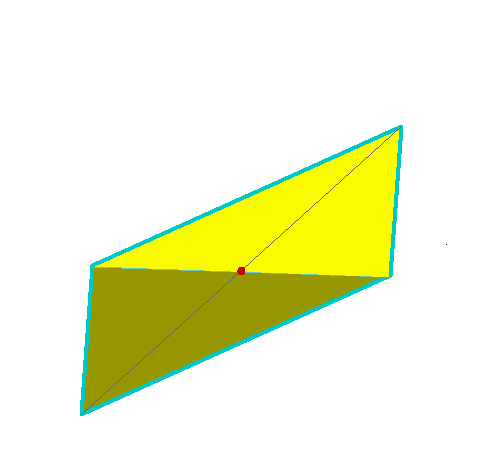
\includegraphics[scale=0.26,trim=10 0 10 53,clip]{./Abrak/Egyeb/NMT1.png}} 
\subfigure[T-Ny\'ujt\'as\ $(T_2: \alpha=2.5).$]{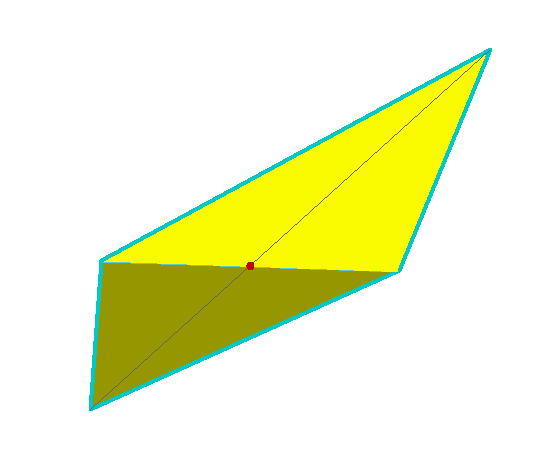
\includegraphics[scale=0.26,trim=10 0 10 53,clip]{./Abrak/Egyeb/NMT2.png}}
\subfigure[T-\"Osszeh\'uz\'as\  $(T_3:  \alpha=1.5).$]{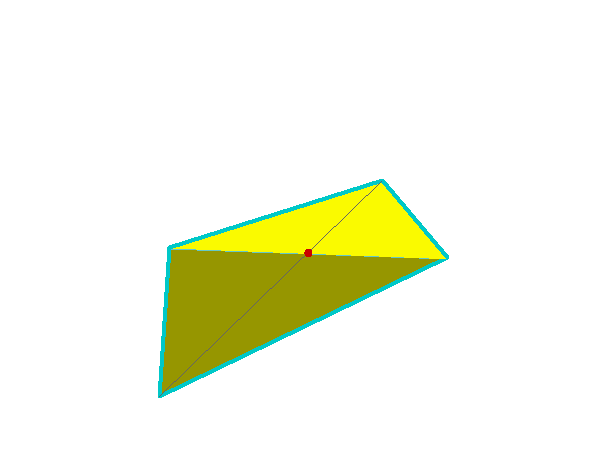
\includegraphics[scale=0.26,trim=10 0 10 53,clip]{./Abrak/Egyeb/NMT3.png}} 
\subfigure[Összeh\'uz\'as\ $(T_4: -1<\alpha<0).$]{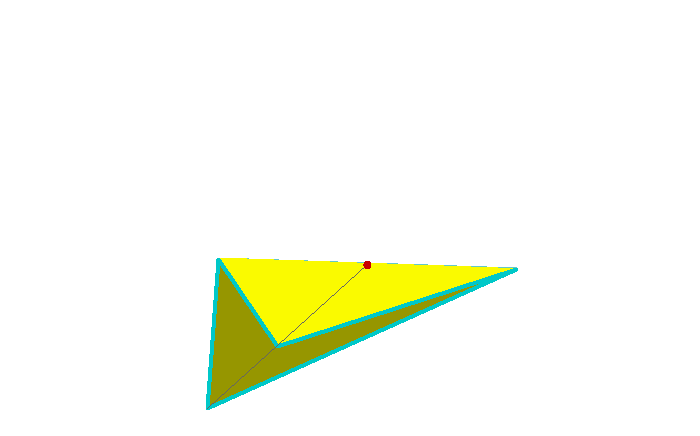
\includegraphics[scale=0.26,trim=10 0 10 185,clip]{./Abrak/Egyeb/NMT4.png}}
\subfigure[Kicsiny\'\i t\'es  $x_3$-b\'ol $(T_5).$]{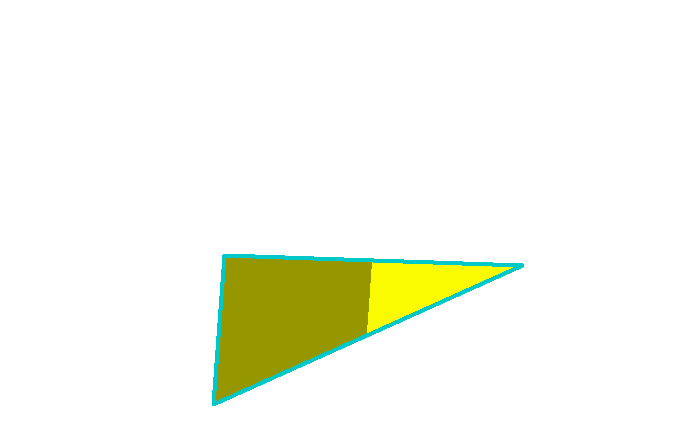
\includegraphics[scale=0.26,trim=10 0 10 185,clip]{./Abrak/Egyeb/NMT5.png}}
\caption{A $Nelder-Mead$ szimplex transzformációi.}
\label{fig:nmtrf}
\end{figure}

Megjegyezzük, hogy a $Nelder-Mead$ szimplex módszer is egy determinisztikus algoritmus. Az algoritmus gyors, hiszen minden lépésben csak néhány függvénykiértékelést kell végezni. Továbbá, a gradiens módszerrel ellentétben az olyan patologikus függvények optimumát is képes gyorsan megtalálni, mint amilyen a Rosenbrock függvény. 


\section{Kvadrat\'ura formul\'ak}
\label{sec:kvad}

A k\"ozel\'\i t\'es hib\'aj\'anak kisz\'am\'\i t\'as\'ahoz k\'etf\'ele kvadrat\'ura formul\'at alkalmazunk
att\'ol f\"ugg\H oen, hogy a dilat\'aci\'os illetve transzl\'aci\'os param\'eterek optimaliz\'al\'as\'at
melyik módszerrel v\'egezz\"uk. Mivel a $Nelder-Mead$, illetve a $PSO$ algoritmusok
csak a f\"uggv\'eny\'ert\'ekekre t\'amaszkodnak, a hibaf\"uggv\'eny \'ert\'ekeinek kisz\'am\'\i t\'as\'ahoz elegend\H o a Hermite-f\"uggv\'enyeket valamilyen feloszt\'as pontjaiban egyszer meghatat\'arozni. Ez implementációs szempontból is fontos, hiszen nem kell minden $(\lambda,a)$ paraméterhez kiszámolni az ettől függő, rekurzióval adott Hermite-féle függvényrendszer tagjait. Ehelyett elég az eredeti diszkrét adatsorozatot dilatálni, illetve eltolni, ami lényegesen kevesebb számítást igényel. Továbbá, az említett feloszt\'as pontjainak valamely Hermite-f\"uggv\'eny z\'erushelyeit v\'alasztva, a hibaf\"uggv\'eny\-ben  szerepl\H o integr\'alok kisz\'am\'\i t\'as\'ahoz
a \cite{waveletECG} dolgozatban haszn\'alt elj\'ar\'ashoz hasonl\'oan kvadrat\'ura formul\'at is alkalmazhatunk. Ennek előnye, hogy az alappontokban a módszer interpolál, így itt lehetséges a jel mintáinak pontos rekonstrukciója. Ugyanakkor, a kapott approximáció is pontosabb, amit a \cite{waveletECG}-ben közölt numerikus tesztek is alátámasztanak.
	\par Mivel a leggyosrabb ereszked\'es m\'odszer\'enek az alkalmaz\'as\'ahoz 
sz\"uks\'eg\"unk van a f\"uggv\'eny parci\'alis deriv\'altjaira, így ezek el\H o\'all\'\i t\'as\'aval
k\"ul\"on  kell foglalkozni. Az Hermite-f\"uggv\'enyek deriv\'altjaira vonatkoz\'o formul\'ak alapj\'an a
parci\'alis deriv\'altakra a hibaf\"uggv\'enyhez hasonl\'o ell\H o\'all\'\i t\'as adhat\'o. Ebben az esetben az \eqref{eq:dotprod} egyenletben szereplő integr\'alok kisz\'am\'\i t\'as\'ahoz ekvidisztans feloszt\'ast alkalmaztunk.

\chapter{EKG jelek tömörítése}
	
	Mindhárom optimaliz\'aci\'o eset\'en, a t\"om\"or\'\i t\H o
elj\'ar\'as el\H ok\'esz\'\i t\'ese megegyezik. A program ind\'\i t\'asakor az els\H o feladat,
hogy a teljes EKG jelet szív\"ut\'esekre bontsunk, majd
minden sz\'\i v\"ut\'est param\'eterk\'ent adjunk tov\'abb a t\"om\"or\'\i t\H o elj\'ar\'asnak. Inicializ\'alni kell tov\'abb\'a
a t\"om\"or\'\i t\H o f\"uggv\'enyek \'altal visszaadott, az aktuális sz\'\i v\"ut\'esre vonatkoz\'o Fourier-egy\"utthat\'okat, 
az approxim\'aci\'o hib\'aj\'at, illetve az optimaliz\'aci\'os elj\'ar\'asok \'altal meghat\'arozott dilat\'aci\'os \'es 
transzl\'aci\'os param\'etereket t\'aroló t\"omb\"oket. \par
	
A t\"om\"or\'\i t\'es el\H ok\'esz\'\i t\'ese nem \'er v\'eget a jel sz\'\i v\"ut\'esekre t\"ort\'en\H o felbont\'asakor. A szívütéseket normalizáljuk is. Ez azt jelenti, hogy az els\H o \'es utols\'o helyen felvett \'ert\'ekeket \"osszek\"ot\H o egyenest kivonjuk a jelb\H ol. Ezt az eljárást az irodalomban az alapvonal eliminálásnak nevezik. Ennek eredm\'enyek\'ent a jel tart\'oja a kezd\H o \'es a v\'egpont \'altal meghat\'arozott intervallum. Végül, a szívütést norm\'aljuk, vagyis az egyes \'ert\'ekeket 
elosztjuk az abszolút maximummal. \par
	A t\"om\"or\'\i t\'es megkezd\'ese el\H ott inicializ\'aljuk a f\"uggv\'enyrendszert, 
melynek során az egyes bázisf\"uggv\'enyek \'altal felvett \'ert\'ekek egy m\'atrix soraiba ker\"ulnek: 
\begin{equation*}
	\Phi:=\left[\Phi_n(\alpha_m)\right]_{0\leq n < N,\;0\leq m < M}\,.
	\label{eq:phi_matrix}
\end{equation*}
A $\Phi\in\mathbb{R}^{N\times M}$ mátrix segítségével az $f\in\mathbb{R}^M$ diszkrét jel Fourier-együtthatói könnyen meghatározhatók:
\begin{equation*}
	c_n:=\left\langle f, \Phi_n \right\rangle=\frac{1}{M} \Lambda^{-1} \Phi f \quad (0\leq n < N)\,,
	\label{eq:phi_coeffs}
\end{equation*}
ahol $\mathbb{R}^{N\times N}\ni\Lambda=\Phi \Phi^T$ Cristoffel-Darboux sz\'amokat tartalmazza. Az előállításban szereplő $\alpha_n\in\mathbb{R}\, (0\leq n < N)$ számokat a \ref{sec:kvad} fejezetnek megfelelően kétféleképpen határoztuk meg. Egyrészt a $PSO$ és $Nelder-Mead$ algoritmusokban a $\Phi_N$ függvény gyökeit véve kvadratúra formulákat definiáltunk. Másrészt a gradiens módszerhez $f$ tartóján egyenletes alapponterndszert használtunk. Felhívjuk a figyelmet arra, hogy az előbbi esetben a gyökök pontos meghatározása kritikus a feladat szempontjából. A probléma megoldásához a \cite{gautschi} könyv által javasolt numerikus eljárást követjük. Nevezetesen, a $H_n$ Hermite-polinom \eqref{eq:identities} rekurziójában szereplő együtthatókat egy tridiagonális mátrixba rendezzük. Könnyen belátható, hogy az $\alpha_n$ gyökök megegyeznek ezen tridiagonális mátrix sajátértékeivel.  \par

Hátra van még a megfelelő $(a,\lambda)$ paraméterek beállítása. Annak érdekében, hogy a reprezentáció minél adaptívabb legyen, több  optimális transzlációt, illetve dilatációt fogunk meghatározni. Az eredeti $f\in\mathcal{F}$ jelet tehát a következő alakban közelítjük:
\begin{equation*}
	S_{\mathbf{n}}^{\mathbf{a},\boldsymbol{\lambda}}f:=\sum_{i=1}^N\sum_{k=0}^{n_i} \langle f^{a_i,\lambda_i},\Phi_{k}\rangle\Phi_{k} \quad
	(a_k \in \Bbb R,\lambda_k>0)\,,
\end{equation*}
ahol $\mathbf{a}=a_1, a_2, \ldots, a_N$ az alkalmazott transzlációk, $\boldsymbol{\lambda}=\lambda_1, \lambda_2, \ldots, \lambda_N$ pedig a dilatációk sorozata. Az egyes sorfejtésekhez tartozó együtthatók számát az $\mathbf{n}=n_1, n_2, \ldots, n_N$ vektor jelöli. Mivel az EKG jel alapvetően három fő hullámból áll ezért esetünkben $N=3.$ Továbbá a \cite{hexp3} dolgozat eredm\'enyei alapj\'an
a QRS komplexumot egy heted, a T hull\'amot hatod, a P hull\'amot pedig egy m\'asodfok\'u ortogon\'alis rendszer seg\'\i ts\'eg\'evel approxim\'aljuk azaz $\mathbf{n}=7,6,2\,.$ Felhívjuk a figyelmet, hogy a legjobb approximáció előállításához a \eqref{eq:hilaprx} egyenlettel ellentétben már az eredeti függvény $f^{a_i,\lambda_i}$ transzformáltját használjuk. Ez nem jelent megszorítást az eredeti problémára nézve, implementációs szempontból viszont $f^{a_i,\lambda_i}$ kiszámítása gyorsabb, mint a $\Phi_n^{a_i,\lambda_i}$ rendszer előállítása.

\section{Matching pursuit algoritmus}

A $(a_i,\lambda_i)$ paraméter párok optimalizációját egymástól függetlenül végezzük. Így azonban nem garantált, hogy az algoritmus a P, QRS, T hullámokat külön-külön approximálja. A probléma megoldására az irodalomban jól ismert ún. $Matching\ Pursuit$ $(MP)$ konstrukciót \cite{mpurs} alkalmazzuk. Ez egy mohó algoritmus, mely minden lépésben a \eqref{eq:Fnfuggv} egyenletben definiált $F_n(a_i,\lambda_i)$ függvény maximalizálására törekszik. Az iteráció $i.$ lépése a következő alakban írható fel:
\begin{equation}
	s^{(i)}=s^{(i-1)} + S^{a_i,\lambda_i}_{n_i} R^{(i-1)} \quad (1\leq i \leq N)\,,
\label{eq:mpurs}
\end{equation}
ahol $R^{(i)}=f-s^{(i)}$ a rezidum függvényt jelöli. Röviden tehát az $s^{(0)}=0,\ R^{(0)}=f$ inicializálás után, az eljárás $i.$ lépésében megkeressük az $R^{(i-1)}$ függvény $\ell^2$ norma szerinti legjobb közelítését, amit ki is vonunk az említett rezidum vektorból. Ezt $N$ iteráción keresztül ismételjük az aktuális $R^{(i)}$ függvényre. Az MP módszer egy gyors algoritmus, mellyel megkonstruálható az $f\in\mathcal{F}$ jel ritka reprezentációja. Emellett lehetséges az EKG szívütéseinek automatikus szeparációja is, hiszen a jel k\"ul\"onb\"oz\H o r\'eszeit eltérő ortogon\'alis rendszerek seg\'\i ts\'eg\'evel k\"ozel\'\i tj\"uk. Felhívjuk a figyelmet arra, hogy az eredeti \cite{hexp3} módszerben ezt a lépést egy külön szegmentáló algoritmus végezte. Így a közelítés jósága erősen függött a szegmentálás eredményétől (lsd. \ref{sec:test} fejezet). A kifejlesztett eljárásnál azonban ez a probléma nem áll fenn még zajos jelek esetén sem. A dolgozatban bemutatott módszer iterációs lépéseit, az $R^{(i)}$ rezidum függvények alakulását, illetve a szeparált EKG jelet az \ref{fig:mpstep} ábra szemlélteti. Jól látható az is, hogy a fekete vonallal jelölt optimális transzláció általában nem az abszolút maximum helyén található. Ez indokolja, hogy a $\lambda_i$ dilatáció mellett az $a_i$ paraméter optimalizációjára is szükség van. Mivel ez utóbbi a kindulásként használt \cite{hexp3} dolgozatból hiányzik, ezért a pontosság és tömörítési arány jelentős javulását várjuk.
\begin{figure}[htb!]
  \centering
\subfigure[A QRS approxim\'aci\'oja.]{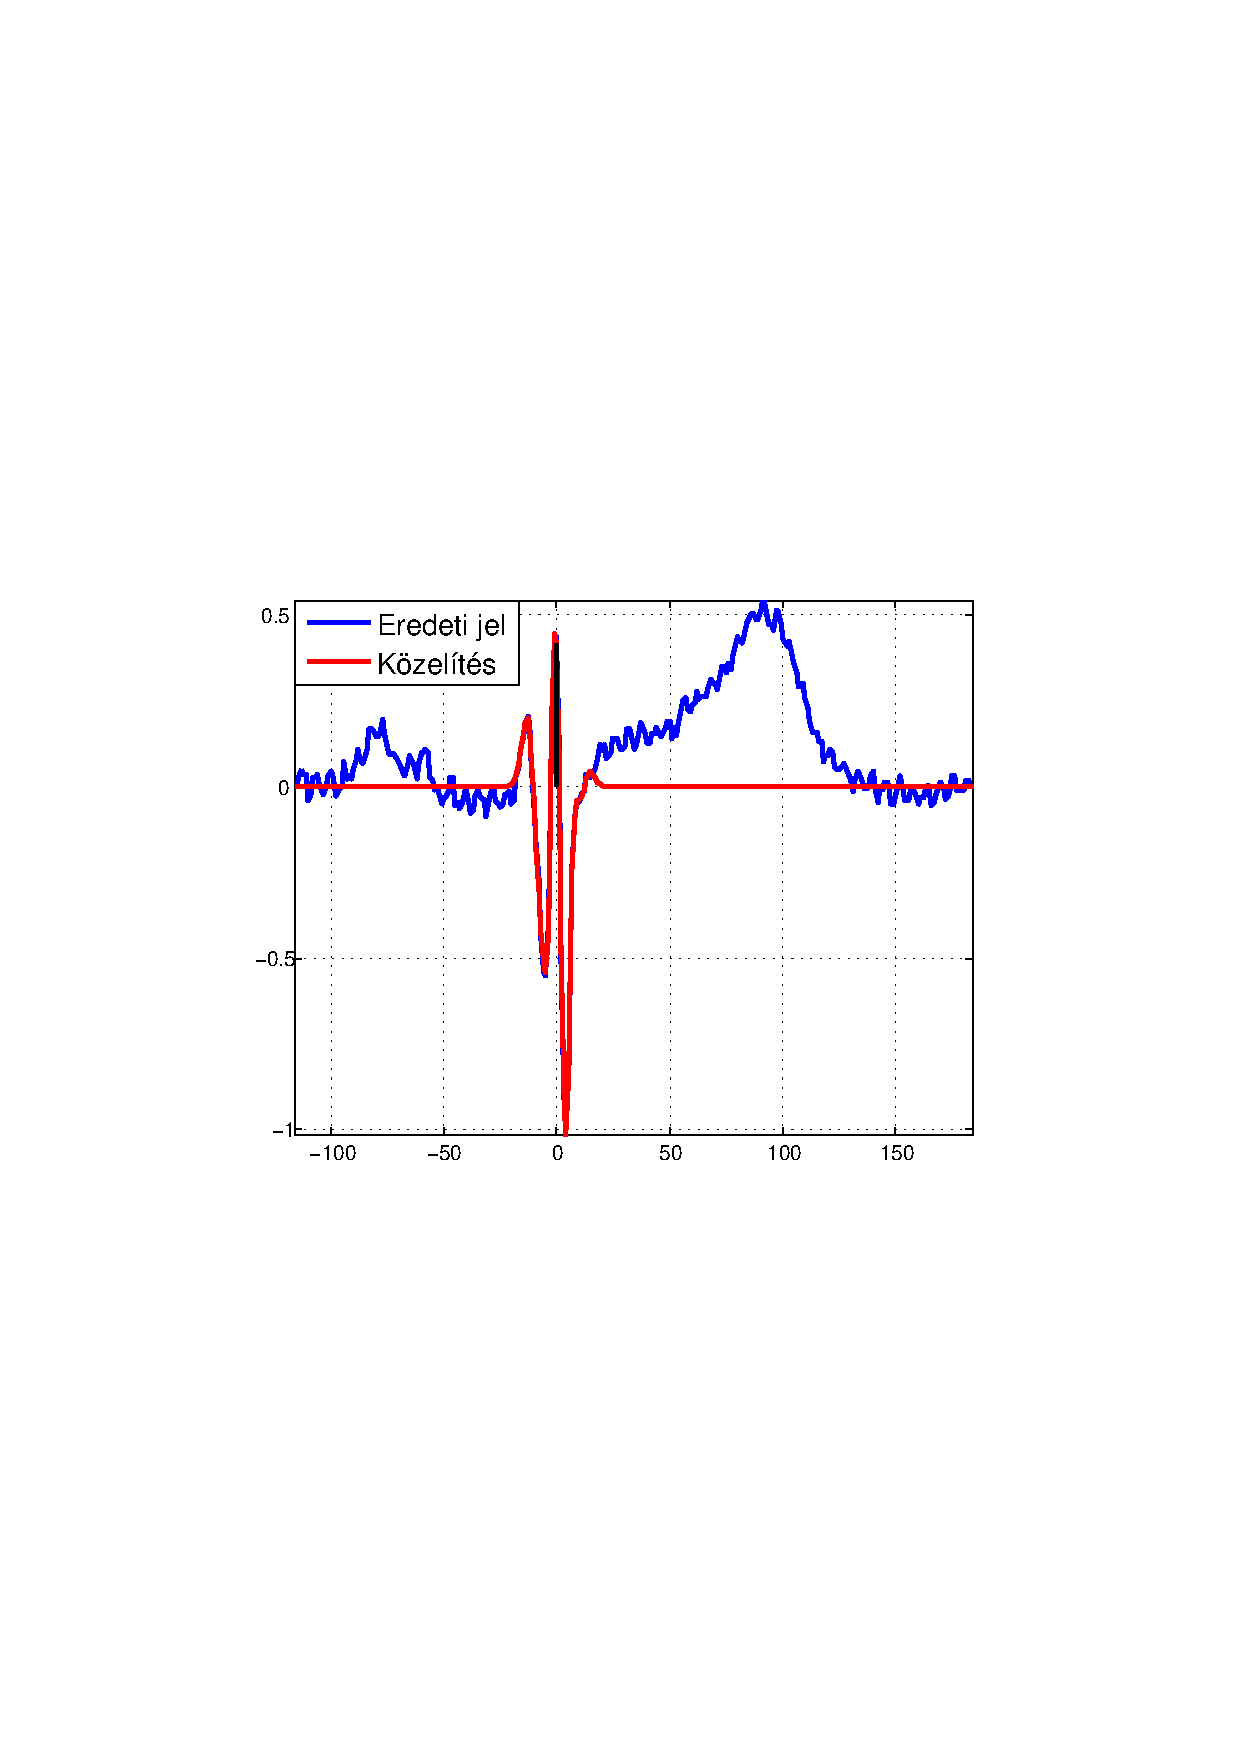
\includegraphics[scale=0.5,trim=120 280 100 280,clip]{./Abrak/Lepesek/abra_lepes0.pdf}} 
\subfigure[A T hull\'am approxim\'aci\'oja.]{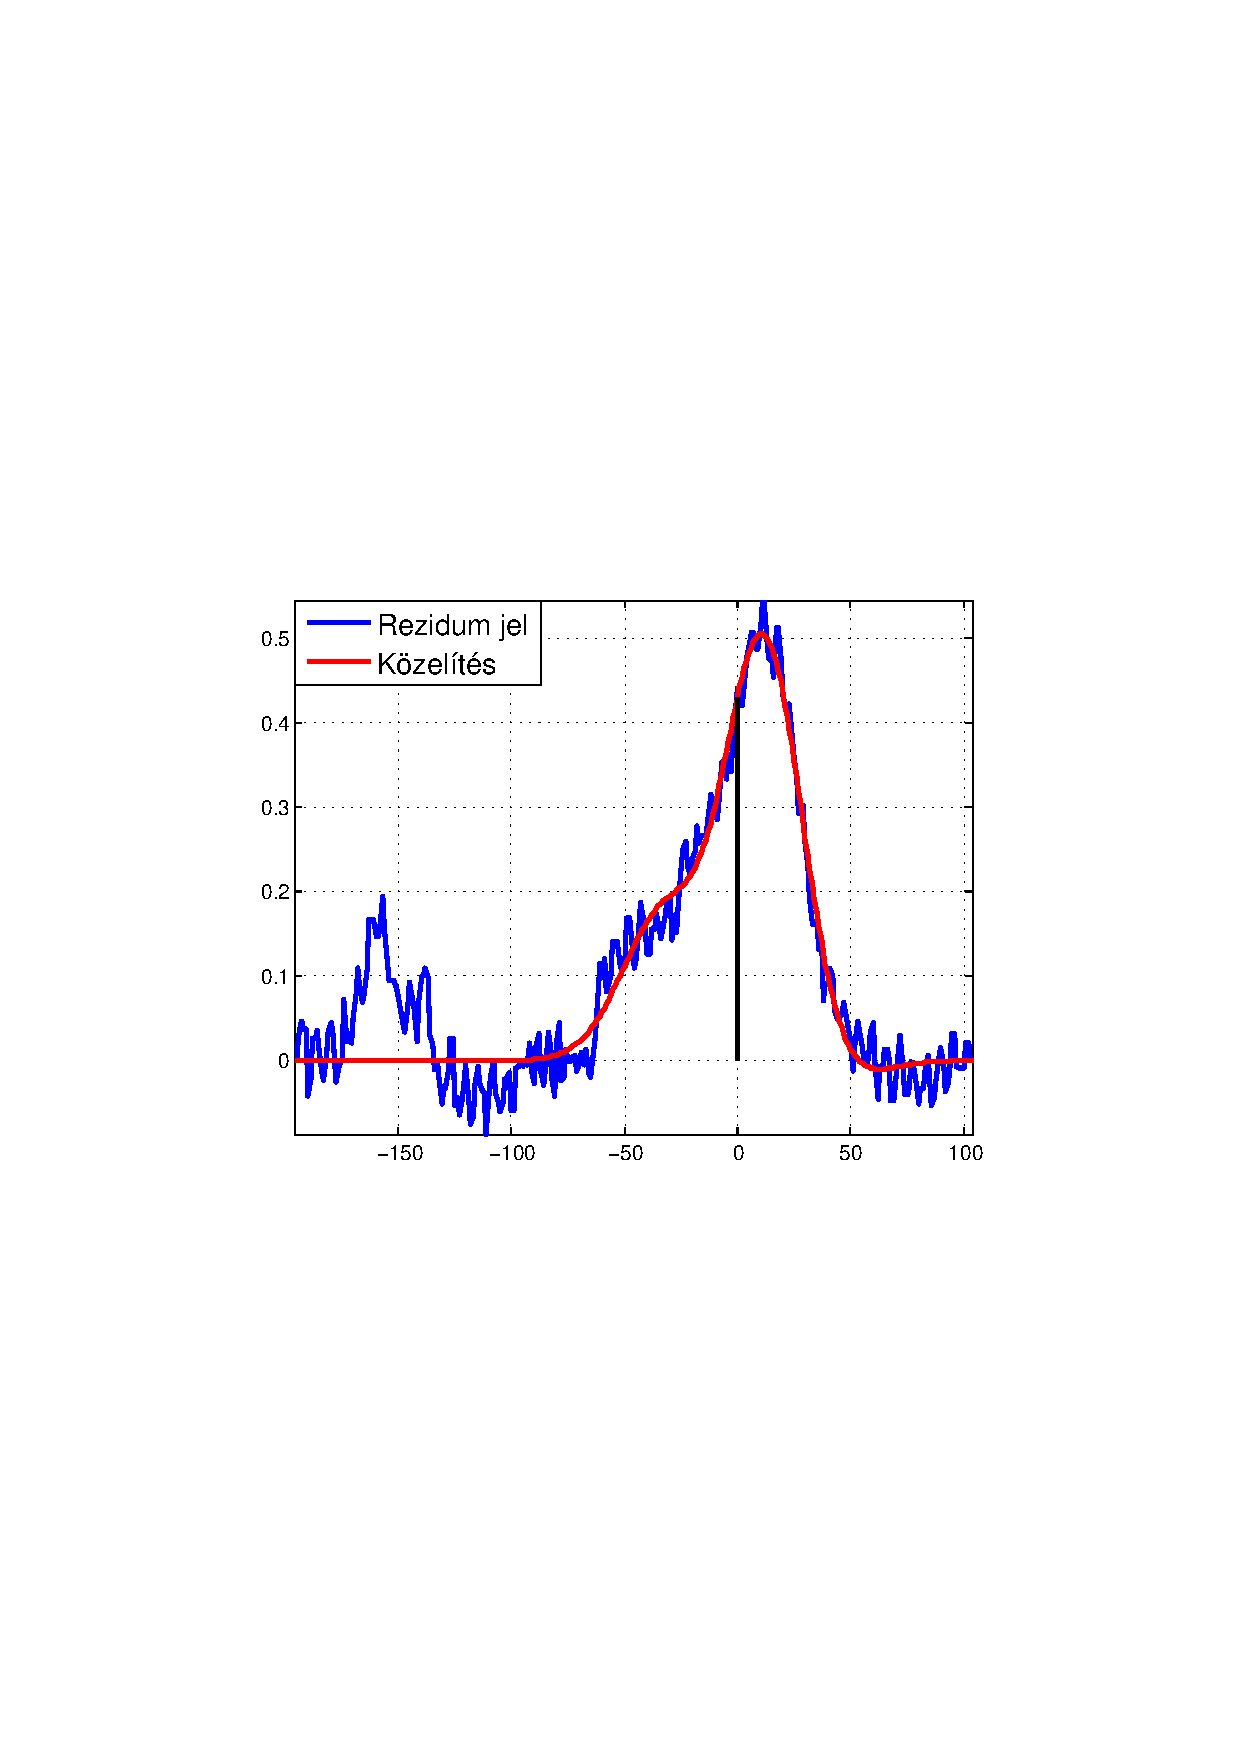
\includegraphics[scale=0.5,trim=120 280 100 280,clip]{./Abrak/Lepesek/abra_lepes1.pdf}}
\subfigure[A P hull\'am approxim\'aci\'oja.]{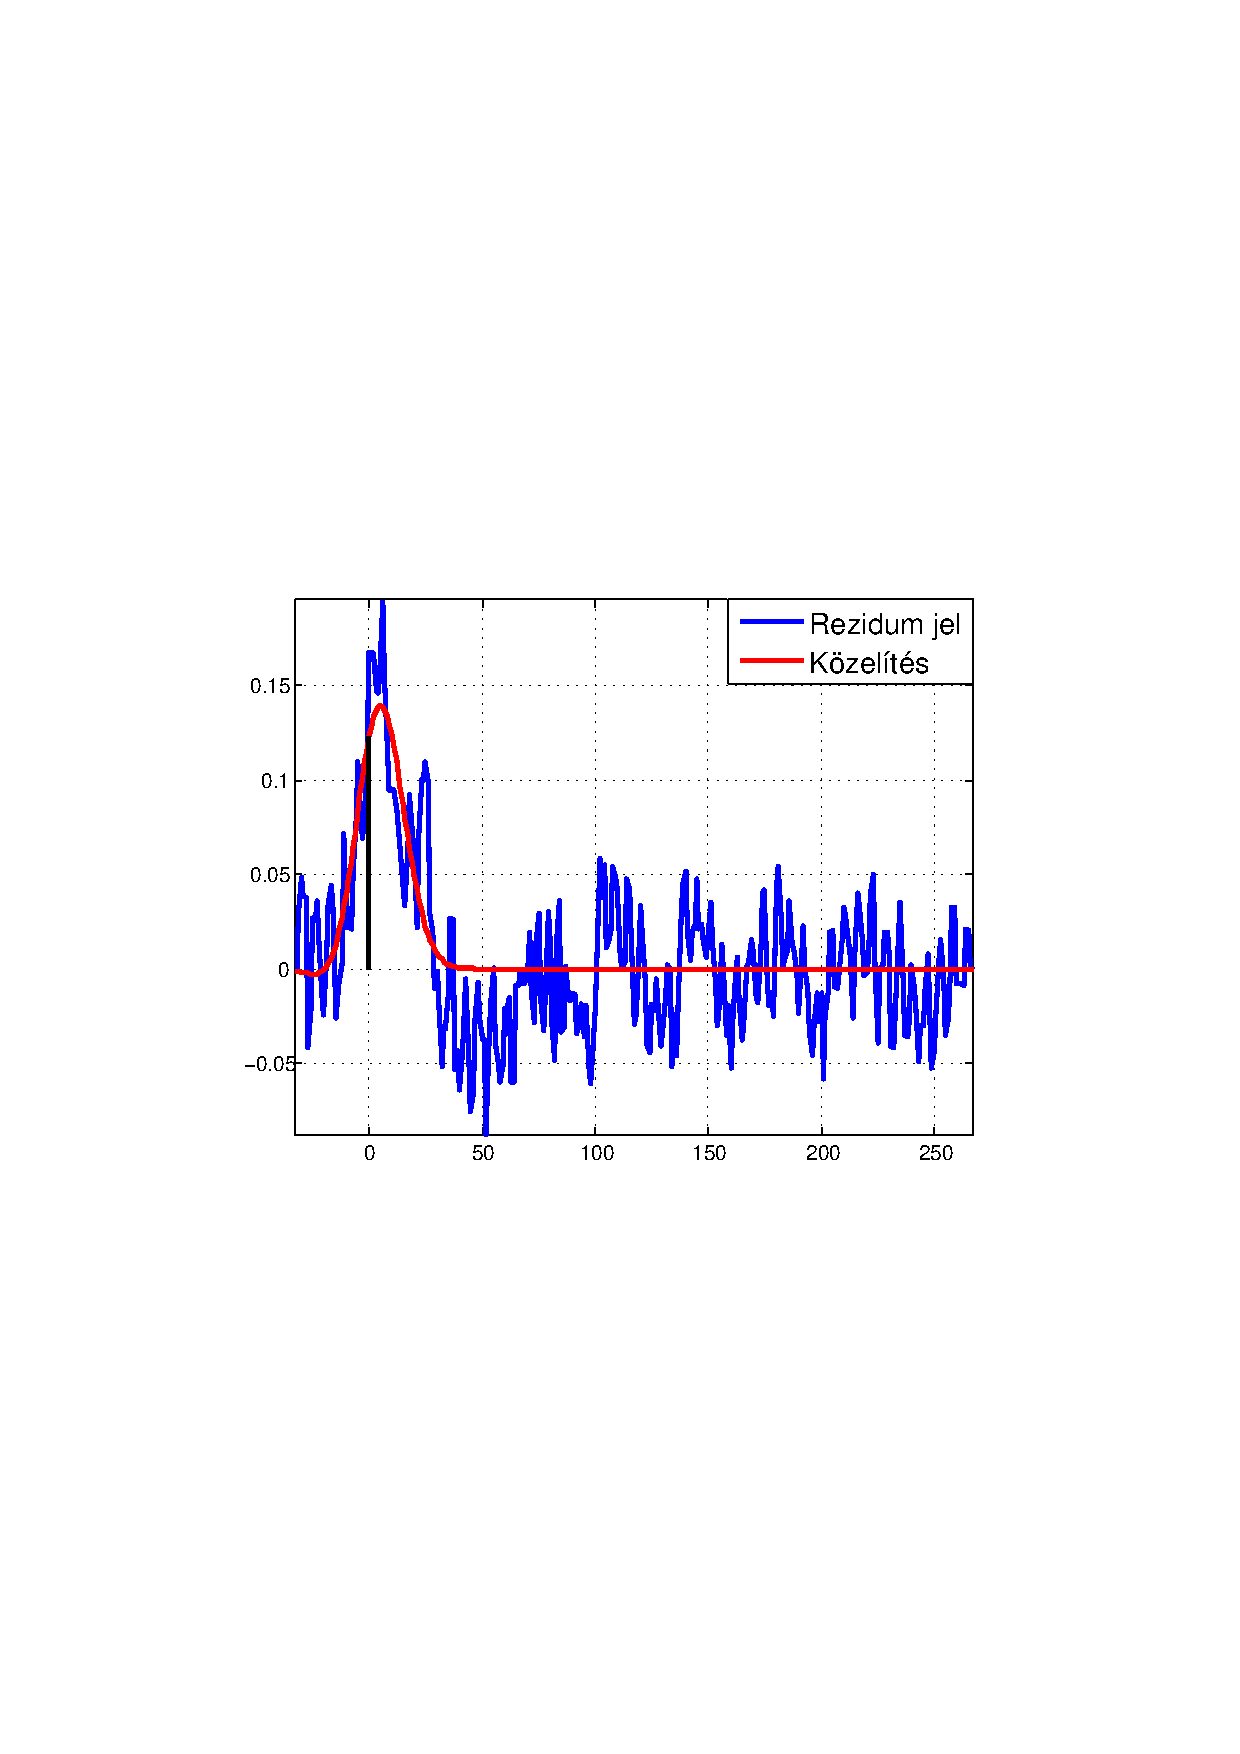
\includegraphics[scale=0.5,trim=120 280 100 280,clip]{./Abrak/Lepesek/abra_lepes2.pdf}} 
\subfigure[Szeparált szívütés.]{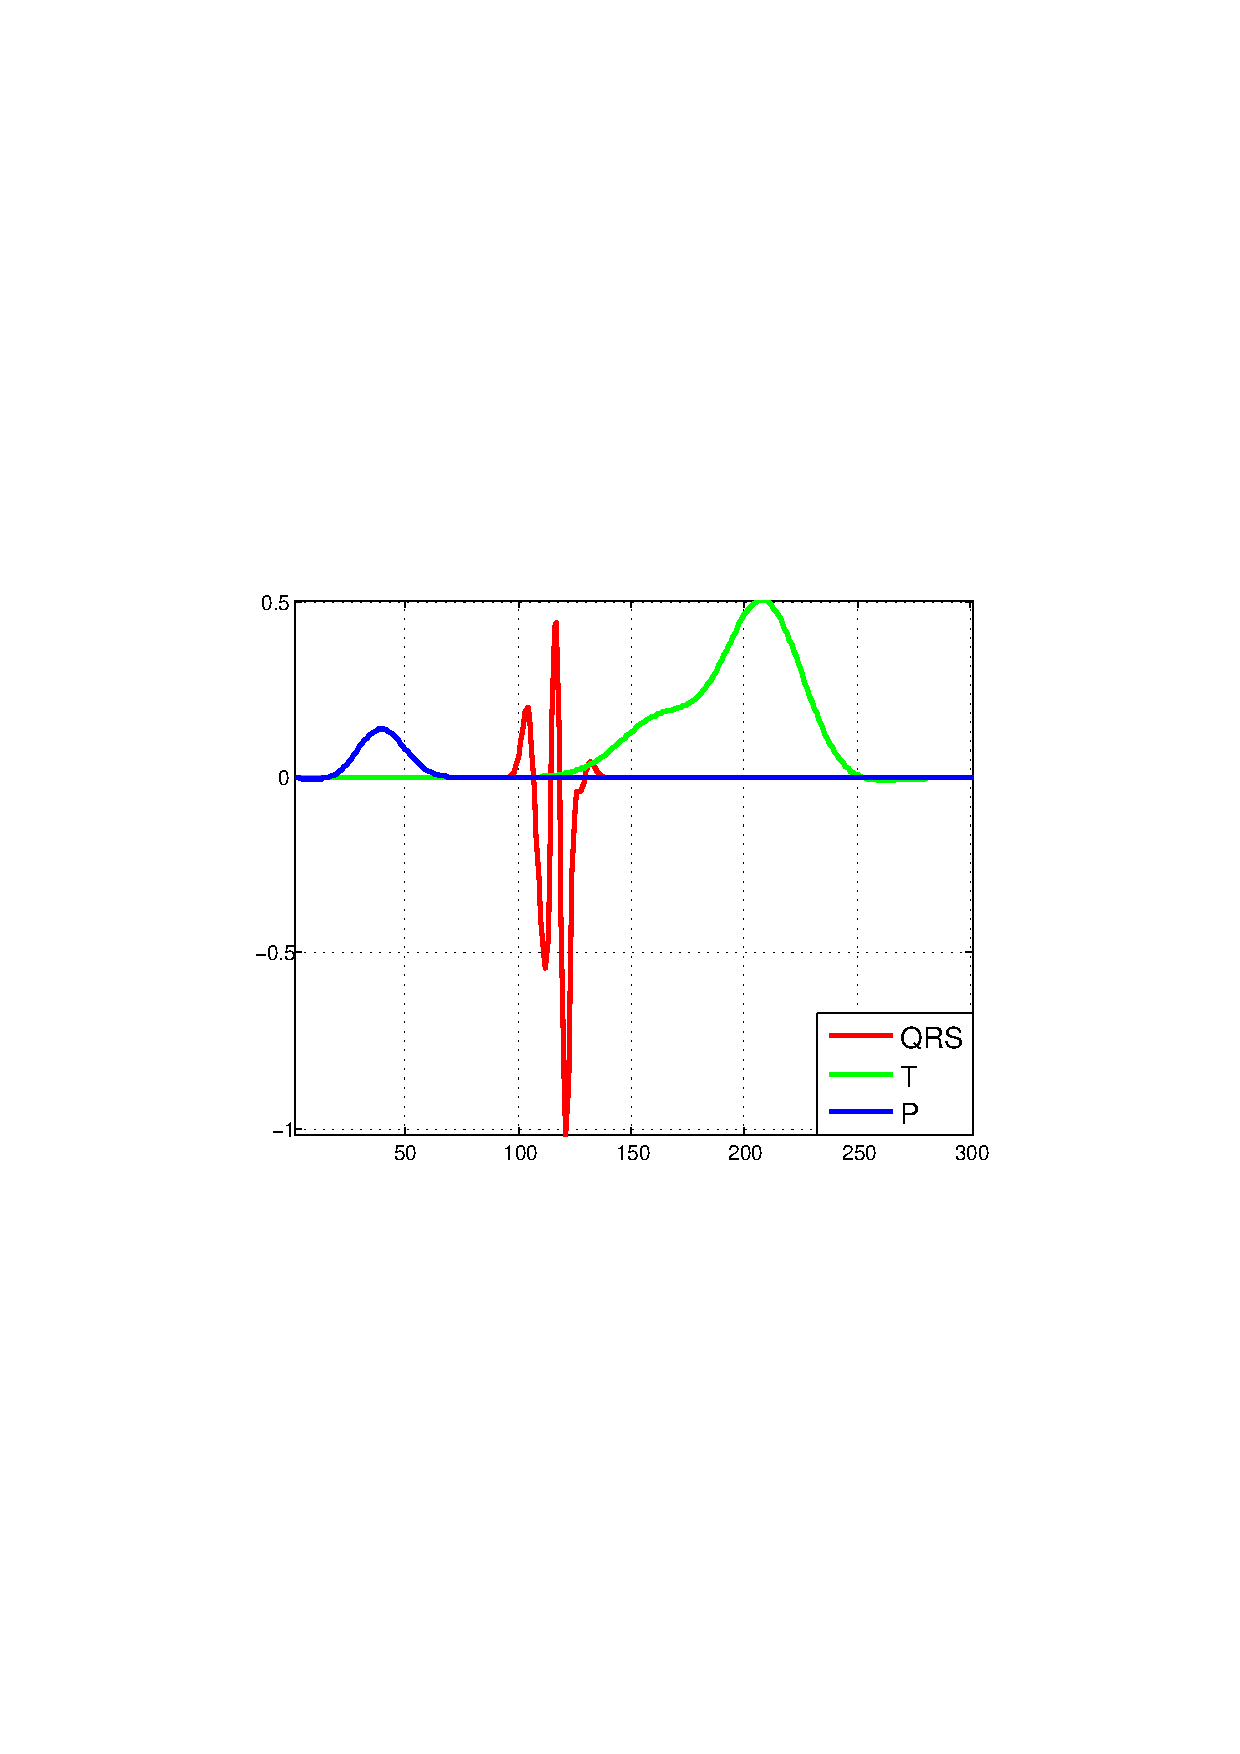
\includegraphics[scale=0.5,trim=120 280 100 280,clip]{./Abrak/Lepesek/abra_lepes3.pdf}}
\caption{Az MP algoritmus lépései.}
\label{fig:mpstep}
\end{figure}

\section{Kvantálás}
Az MP algoritmus által megtalált optimális paramétereket tárolnunk is kell. Mivel a reprezentáció erősen függ az $\mathbf{a}$ transzlációs paraméterek vektorától, ezért ezt annyi biten ábrázoljuk, ami a pontos rekonstrukcióhoz szükséges, így $b=\log_2(\displaystyle{\max_{i}\left|a_i\right|})+1.$ Az egyes hullámokhoz tartózó dilatációk $\boldsymbol{\lambda}$ és $\mathbf{c}=[c_{n}^{(i)}] \; (1\leq n \leq n_i, \, 1\leq i\leq N)$ együtthatók vektorát azonban kerekítve tároljuk. Ehhez a dolgozatban lineáris kvantálást használunk. Jelölje $c_{\max}$ és $c_{\min}$ a $\mathbf{c}$ vektor abszolútértékben maximális és minimális elemét. Ekkor a lineáris kvantálás művelete a következőképpen definiálható:
\begin{equation}
	Q(c):=c_{\min}+\sgn(c) \cdot \Delta \cdot \left\lfloor \frac{\left|c-c_{\min}\right|}{\Delta}+\frac{1}{2}\right\rfloor\,,
\label{eq:quant}
\end{equation}
ahol $\Delta=\left|c_{\max}-c_{\min}\right|/2^{b-1}.$ A $Q(c)$ kerekített értékeket az előjel figyelembevételével $b$ biten tároljuk. A dilatációs paraméterek kvantálását ugyanezen függvény segítségével végezzük el. A $b$ bitek számát tapasztalati úton, tesztek segítségével határoztuk meg. 

A vizsgálatokhoz a PhysioNet \cite{PhysioNet} MIT-BIH EKG adatbázis rekordjait használtuk. Ez $48$ egyenként fél órás valódi EKG jelet tartalmaz, amit $47$ egészséges illetve beteg páciensről gyűjtöttek össze. A rekordok két elvezetése másodpercenként $360$ mintát rögzít 11 bites felbontásban. A tömörítés teszteléséhez az irodalomban gyakran csak a $117$ és $119$ sorszámú rekordokat használják (pl. \cite{jpeg2000ECG, waveletECG}). Ennek az az oka, hogy e két felvétel több abnormális szívütést tartalmaz, így bonyolultságukat tekintve jó tesztrekordok. A vizsgálatok során először kiszámoltuk az említett rekordok szívütéseihez tartozó optimális paramétereket. Majd a pontosan ábrázolt $\mathbf{c}$ együttható és $\boldsymbol{\lambda}$ dilatációs vektorokat egyre csökkenő $b$ bitszámmal újra kvantáltuk. Eközben vizsgáltuk a közelítés pontosságát (PRD) és a tömörítési arányt (CR). Ezek pontos definícióját a \ref{sec:test} fejezetben adjuk meg. A tesztek során a két rekord összesen $1528+1979$ szívütését dolgoztuk fel. Az eredményeket a \ref{fig:quant} grafikonon ábrázoltuk. Jól látható, hogy a közelítés hibája $7$ bit után lényegében nem változik. Ezért a további tesztek során a dilatációs paramétereket és az együtthatókat is $b=7$ biten tároljuk a \eqref{eq:quant} egyenletnek megfelelően.
\begin{figure}[htb!]
\centering
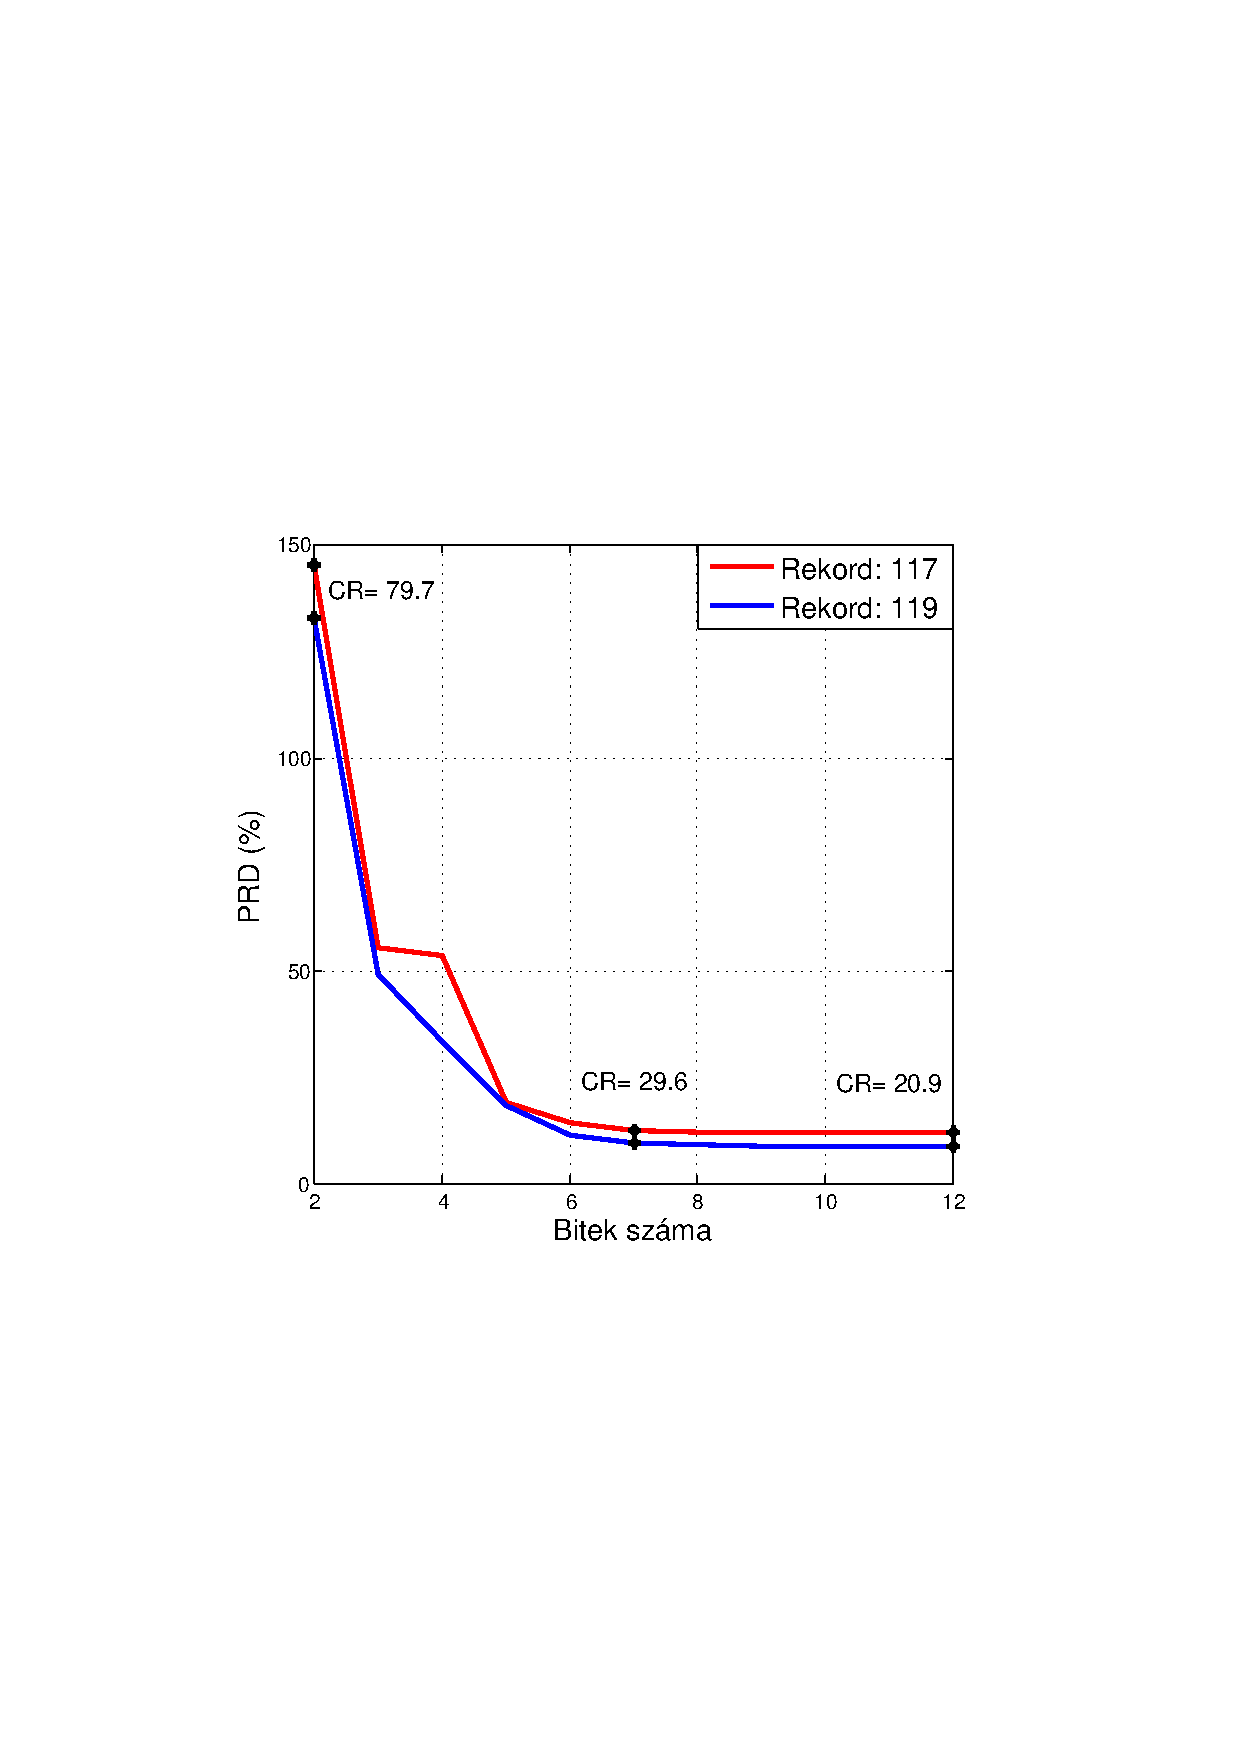
\includegraphics[scale=0.4,trim=100 260 100 255,clip]{./Abrak/Kvantalas/abra.pdf}%
\caption{A rekonstruált 117, 119 rekordok paramétereinek kvantálása.}%
\label{fig:quant}%
\end{figure}

\section{Tesztek, \'es eredm\'enyek}
\label{sec:test}
	A dolgozatban ismertetett algoritmust a 117, 119-es rekordok mellett az MIT-BIH adatb\'azisban egyéb felvételein is lefuttattuk. Így összesen $3$ órányi adaton, $12830$ darab sz\'\i v\"ut\'esen pr\'ob\'altuk ki a m\'odszert. Az összehasonlíthatóság érdekében a tesztet megismételtük az eredeti \cite{hexp3} algoritmussal is. Mindkét esetben a kvantálást $b=7$ biten hajtottuk végre, az egyes szegmenseket pedig $\mathbf{n}=7,6,2$ együtthatóval reprezentáltuk. A futásidő csökkentéséhez a PSO algoritmus rajméretét $10$-re, az iterációk számát pedig 15-re állítottuk be. Így egy $30$ perces rekordon a Nelder-Mead (NM) szimplex módszer átlagosan $1400$ másodpercig, míg a PSO esetén $1600$ másodpercig futott. Megfelelő hardwer konfiguráció esetén ez már valós idejű adatfeldolgozást feltételez. Az eredményeket a pontosság és a tömörítési arány szempontjából is értékeltük:
\begin{equation*}
		\PRD=\frac{\left\|S_{\mathbf{n}}^{\mathbf{a},\boldsymbol{\lambda}}f-f\right\|_2}{\left\|f-\conj{f}\right\|_2}\times 100\,,\qquad  \CR=\frac{\text{eredeti EKG mérete}}{\text{tömörített EKG mérete}}\times 100\,,
		\label{eq:prd_cr}
\end{equation*}
ahol $\conj{f}$ a jel átlaga. A pontosság mérésére az irodalomban az ún. $percentage$ $root$ $mean$ $square$ $difference$ $(PRD)$ terjedt el. Vegyük észre, hogy ez az $\ell^2$ normában mért relatív hibával egyenlő, ami független a jel átlagától. Az algoritmusok összehasonlításánál a CR-t és a PRD-t is figyelembe kell venni. Ez azonban megnehezíti a módszerek értékelését. Ezt kiküszöbölendő, a \cite{pkselect} cikkben bevezették az ún. $Quality\ Score$ $(QS)$ fogalmát, ami a CR és a PRD hányadosa. Így az az algoritmus tekinthető jobbnak, amelyik magasabb QS-el rendelkezik. Ennek megfelelően az eredményeket a \ref{tab:results} táblázatban foglaltuk össze.
\begin{table}[H]
\centering
	\scalebox{0.7}{
\begin{tabular}{|c||cccc|cccc|cccc|}
\multicolumn{1}{c}{} & \multicolumn{4}{c}{\textbf{Hiba (PRD \%)}} & \multicolumn{4}{c}{\textbf{A t\"om\"or\'\i t\'es ar\'anya (CR $1:X$)}} & \multicolumn{4}{c}{\textbf{Quality Score ($\CR:\PRD$)}}\bigstrut\\\hline
\textbf{Rec.} & \textbf{Eredeti} & \textbf{NM} & \textbf{PSO} & \textbf{JPEG2} & \textbf{Eredeti} & \textbf{NM} & \textbf{PSO} & \textbf{JPEG2} & \textbf{Eredeti} & \textbf{NM} & \textbf{PSO} & \textbf{JPEG2} \bigstrut[t]\\
101 & 11.20 & 11.10 & 11.13 &11.07& 29.71 & 27.22 & 27.22 & 18.94 &\textbf{2.65}&2.45&2.47& 1.71\\
117 & 13.20 & 11.81 & 17.66 &11.66& 36.07 & 33.06 & 33.06 & 23.66 &2.73&\textbf{2.79}&1.87& 2.02\\
118 & 19.83 & 17.79 & 16.65 &17.72& 24.34 & 22.30 & 22.30 & 32.91 &1.22&1.25&1.33& \textbf{1.85}\\
119 & 14.27 & 8.76 & 10.20  &8.80 & 27.89 & 25.55 & 25.55 & 23.85 &1.95&\textbf{2.91}&2.51& 2.71\\
201 & 13.51 & 12.17 & 12.17 &12.14& 28.21 & 25.35 & 25.35 & 13.15 &\textbf{2.08}&\textbf{2.08}&\textbf{2.08}& 1.08\\
213 & 19.92 & 18.28 & 17.60 &18.29& 17.08 & 15.64 & 15.64 & 35.23 &0.85&0.85&0.88& \textbf{1.92}\\
%214 & 7.61 & 7.90 & 11.40   &7.91 & 24.53 & 22.04 & 22.47 & 19.32 &&&&\\
\hline
\textbf{\'Atlag} & 14.22 & 12.55 & 13.83 &12.51& 26.83 & 24.45 & 24.51 & 23.86 &1.91&\textbf{2.06}&1.85& 1.88\\\hline
\end{tabular}
}
\caption{A tömörítés \"osszehasonl\'\i t\'asa k\"ul\"onb\"oz\H o m\'odszerek eset\'en.}
\label{tab:results}
\end{table}

Általánosságban elmondható, hogy az összehasonlított módszerek közül, a dolgozatban bemutatott algoritmus volt a leghatékonyabb. Utóbbi PRD-je átlagosan $2\%$-al jobb, mint az eredeti módszeré. A tömörítési arány egy kicsit rosszabb, ami várható hiszen a transzlációs paramétereket is tárolnunk kell ellentétben \cite{hexp1}-el. Végeredményben viszont az átlagos QS alapján a dolgozatban bemutatott és a Nelder-Mead optimalizációval kombinált módszerünk győzött. Továbbá vegyük észre, hogy a $119$-es rekord esetén jelentős különbség van a két módszer között. A jelenség megértéséhez tekintsük a \ref{fig:eredetiVSsajat} ábrát, ahol a kérdéses jel első szívütését rajzoltuk ki. Látható, hogy az eredeti algoritmussal adott approximáció a T hullám közelében nagyon rossz. Ez egyrészt a szegmentáló algoritmus hibájának, másrészt a transzlációs paraméter hiányának köszönhető. Az eredeti algoritmus az EKG jelet a zöld pontokkal megjelölt szakaszokon közelíti, ahol az alkalmazott Hermite-függvények az intervallum középre vannak igazítva (lsd. fekete vonalak). Mivel a T hullám asszimetrikusan helyezkedik el az adott szegmensen, így még elég nagy dilatáció esetén sem lehet kompenzálni a hibát. A kidolgozott módszer azonban a $(a_i,\lambda_i)$ szabad paramétereknek és az optimalizációnak köszönhetően képes megbírkózni a feladattal és közel kétszer alacsonyabb PRD-vel állítja elő a jelet. Megjegyezzük, hogy ehhez mindkét reprezentációban ugyanannyi együtthatót használtunk fel. A saját módszerünk tárolás szempontjából csupán abban különbözik, hogy szegmensenként szükség van plussz egy transzlációs paraméterre. A példából érthető az is, hogy a \ref{tab:results} táblázat bizonyos rekordojain az eredeti algoritmus miért teljesít majdnem olyan jól, mint a dolgozatban bemutatott módszer. Ha ugyanis normális szívütéseink vannak és a szegmentálás is pontos, akkor az intervallumok felezőpontja közel van az optimumhoz. Mivel ez valós jelek esetén egyáltalán nem garantált, így a dolgozat problémafelvetése jogos és az erre adott megoldás gyakorlati szempontból is értékelhető.
\vspace{5mm} 
\begin{figure}[htb!]
  \centering
\subfigure[Eredeti módszer.]{\includegraphics[scale=0.55,trim=120 280 100 280,clip]{./Abrak/Eredeti_Hermite/abra1.pdf}}\hspace{5mm}
\subfigure[Saját módszer.]{\includegraphics[scale=0.55,trim=120 280 100 280,clip]{./Abrak/Sajat_Hermite_Nelder_Mead/abra1.pdf}}
\caption{Asszimetrikus EKG jel közelítése.}
\label{fig:eredetiVSsajat}
\end{figure}
 	
Eredményeinket szerettük volna összevetni más, az irodalomban gyakran hivatkzott módszerekkel is. Ehhez a \cite{jpeg2000ECG} cikkben bemutatott 2D-s algoritmust használtuk. Választásunkat a módszer egyszerűsége, illetve az alkalmazott JPEG 2000 szabvány elterjedése indokolja. Az algoritmus az EKG jelek szegmentálása után az R hullám mentén rendezi a szívütéseket a \ref{fig:jpegECG} ábrának megfelelően. Mivel a szívütések hossza eltérő, ezért előbb ezeket ki kell egyenlíteni, például a végpontok ismétlésével. Az így kapott egyenlő hosszú szívütések vektorait mátrixba rendezve egy képet kapunk, melyet a JPEG 2000 veszteséges képtömörítővel tárolunk. Az PhysioNet rekordjain kapott eredményeket a \ref{tab:results} táblázat utolsó oszlopa tartalmazza. Ez esetben a paramétereket úgy állítottuk be, hogy a pontosság közel legyen a saját módszer PRD-jéhez. Így az eredmények értékelése egyszerűbb. Az átlagos CR alapján az általunk kidolgozott módszer jobbank bizonyult. Mivel a JPEG 2000 szabvány egy wavelet alapú algoritmust használ, a tömörítési arány várhatóan ott lesz magas ahol a szívütésekből készített kép sima, homogén tartományokat tartalmaz. Így fordulhatott elő, hogy a $118$ és $213$ rekordok esetében kiugróan magas CR értékeket kaptunk.
\begin{figure}[htb!]
  \centering
\subfigure[A QRS-hez igazított szívütések.]{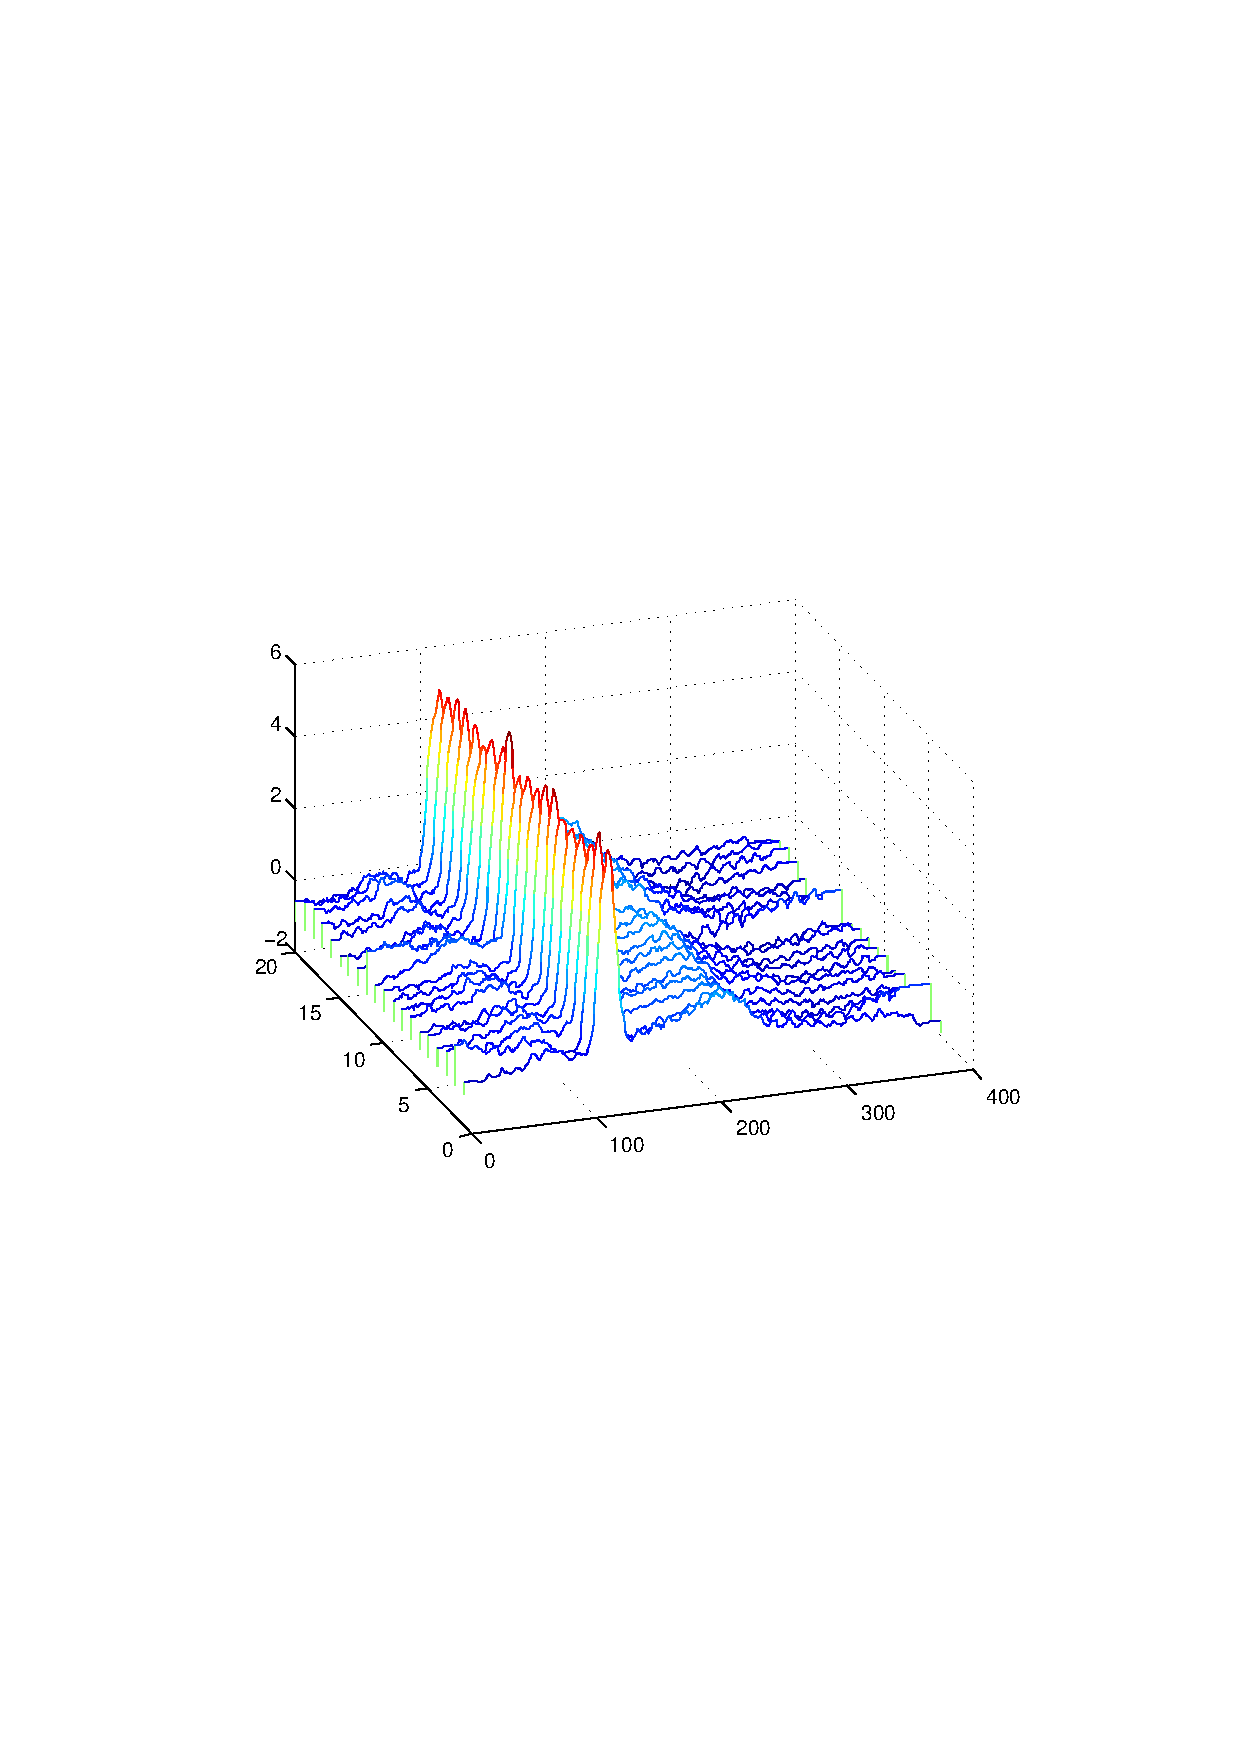
\includegraphics[scale=0.5,trim=100 280 100 280,clip]{./Abrak/2D_JPEG_lepesek/waterfall_ECG.pdf}}
\subfigure[Szívütések felülnézete, tömörítendő kép.]{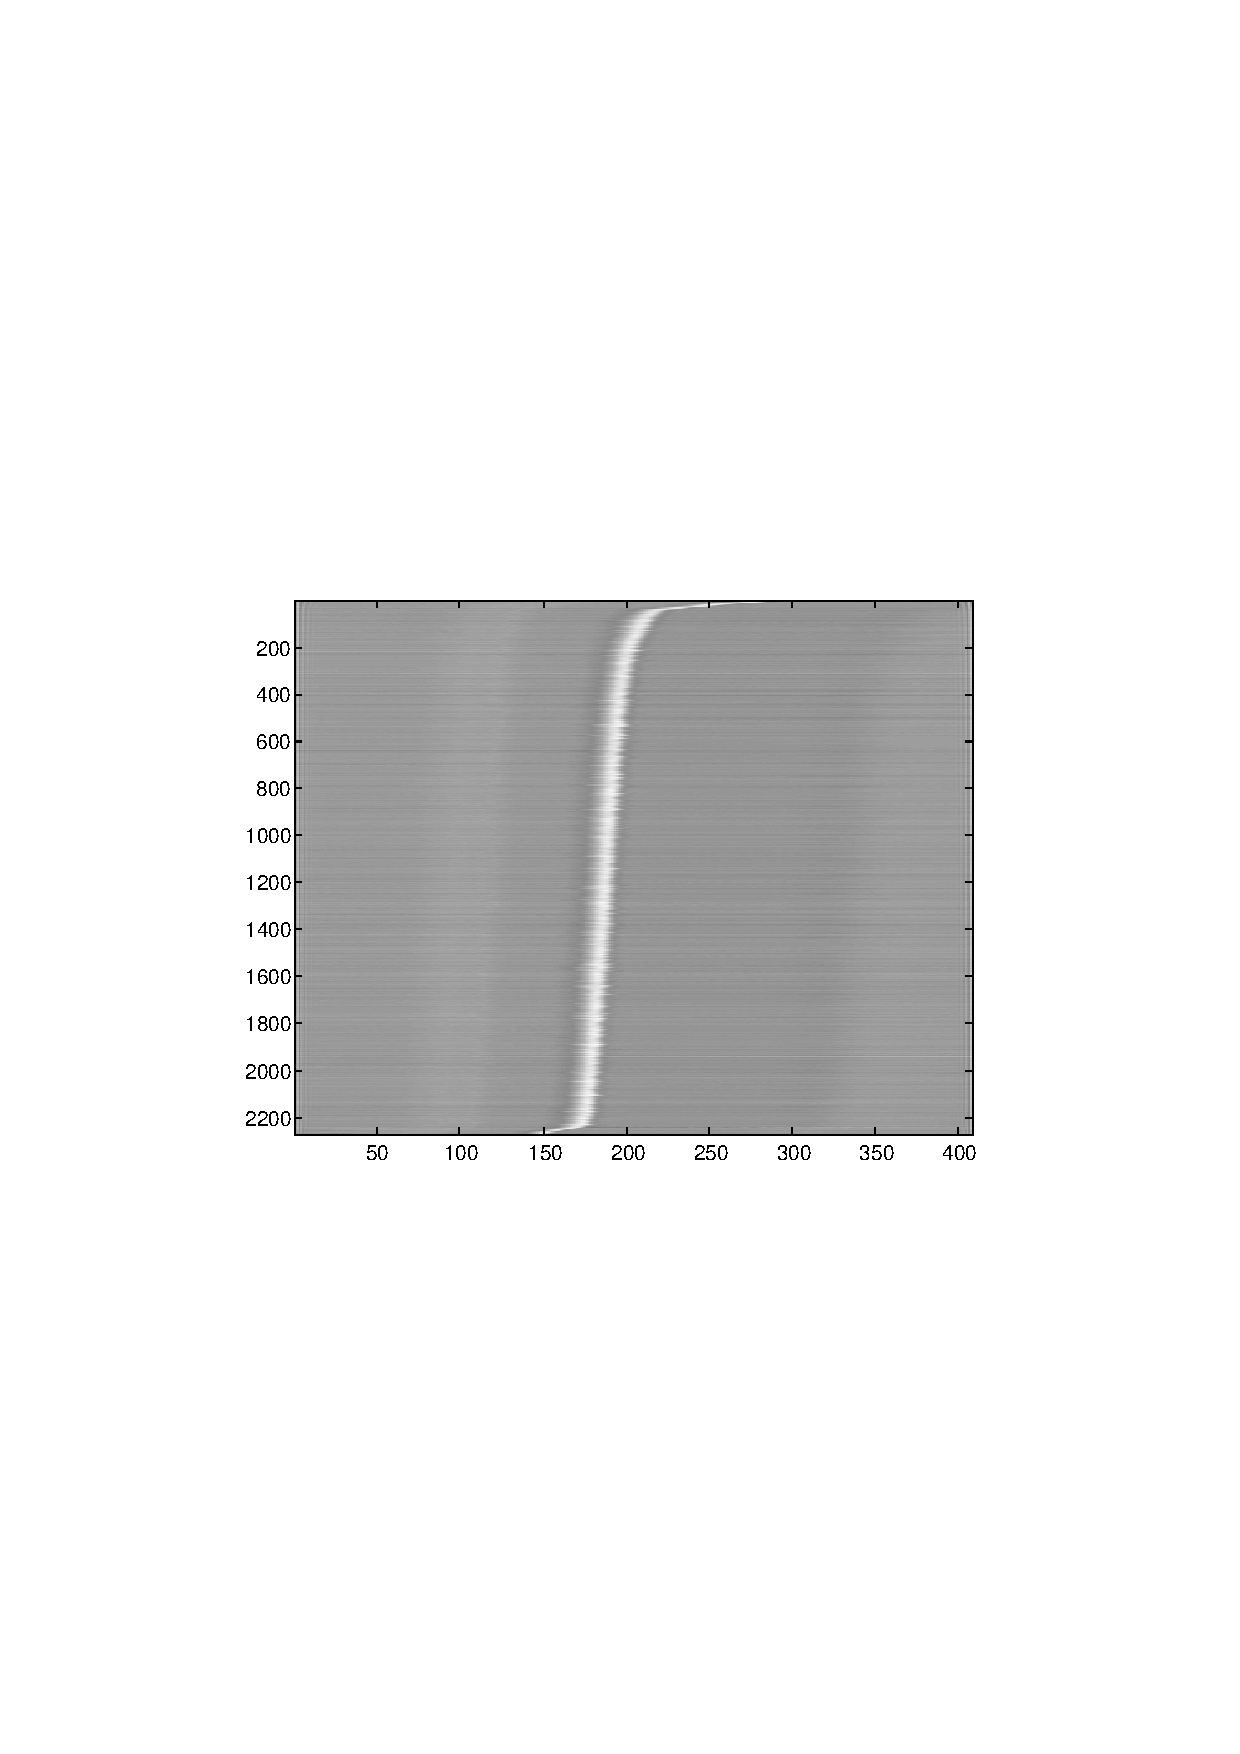
\includegraphics[scale=0.5,trim=100 280 100 280,clip]{./Abrak/2D_JPEG_lepesek/ecg2d.pdf}}
\caption{EKG jelek tömörítése a JPEG 2000 képtömörítő algoritmussal.}
\label{fig:jpegECG}
\end{figure}	
Végül megjegyezzük, hogy a teszteléshez felhasznált módszerek mindegyikében szükséges az EKG jelek legalább szívütésenkénti szegmentálása. A PhysioNet MIT-BIH adatbázisa kardiológusok által annotált EKG jeleket tartalmaz. Ez azt jelenti, hogy a szívütések QRS komplexusait orvosok korábban kézzel bejelölték. Ugyan az annotációkat a tesztek során felhasználtuk, de ez nem csökkenti a módszer robosztusságát. A szegmentáláshoz használhatjuk például az irodalomban gyakran hivatkozott Pan--Tompkins-féle QRS detektort is \cite{tompkins}.

\chapter{Összefoglalás, kitekintés}
A dolgozatban a \cite{hexp3, hexp5} cikkekben bemutatott algoritmusokból kiindulva egy új EKG tömörítő eljárást konstruáltunk. Az módszer adaptív, amit a Hermite-függvények argumentum transzformációjával értünk el. A reprezentáció szabad $(a_i,\lambda_i)$ transzlációs és dilatációs paramétereit három optimalizációs algoritmussal állítottuk elő. A módszerek előnyeit, hátrányait egyaránt figyelembe vettük az alkalmazás során. Az említett optimum létezését beláttuk, illetve a gradiens módszerhez szükséges parciális deriváltakat levezettük. A tömörítő algoritmus hatékonyságát a PhysioNet adatbázis valós EKG felvételein teszteltük. A numerikus vizsgálatokban összesen $3.5$ órányi rekordot dolgoztunk fel, ami biztosította statisztikai kisérletekhez szükséges magas mintaelemszámot. Ezek alapján megállapítható, hogy a kiindulásként felhasznált \cite{hexp3, hexp5} algoritmusok eredményeit megjavítottuk. A \cite{jpeg2000ECG} cikkben ismertetett, JPEG 2000 alapú 2D-s EKG tömörítő eljárást is összehasonlítottuk a dolgozatban implementált módszerrel. Ez esetben is a saját algoritmusunk győzött.

Megjegyezzük azonban, hogy a kidolgozott módszernek is vannak hátrányai. Mivel az iteratív approximáció során az MP megközelítés alkalmaztuk, így örököltük annak hibáit is. Előfordulhat, hogy az első lépésben nem a QRS komplexust közelítjük, hanem a T hullámot. Így az eredetileg ide szánt $7$ együtthatót a $T$ hullámra "pazaroljuk". Ez azonban a helyes inicializálással, illetve a QRS hibájának súlyozásával kiküszöbölhető. Másik probléma, hogy az MP algoritmus egy mohó stratégiát követ a $(a_i,\lambda_i)$ paraméterek meghatározásához. Így előfordulhat, hogy egy iterációban a szívütés egynél több hullámát is közelítjük, ha ez az $\ell^2$ hiba szempontjából indokolt. Ezt szemlélteti a \ref{fig:counterexample} ábra. Jól látható, hogy az első esetben a PRD kisebb, mint a második példában. Előbbinél azonban a rezidum függvény is jóval bonyolultabb. Tehát a végeredmény szempontjából előnyösebb, ha minden lépésben csak egy hullámot közelítünk. A jelenség az MP módszer és a mohó stratégia jól ismert hátránya, melyet a \cite{bpurs} dolgozat is részletesen tárgyal. Eszerint a probléma mérsékelhető, ha az mohó stratégiát más módszerekre cseréljük. Megjegyezzük, hogy ez úgy is megoldható, hogy az iterációs megközelítés helyett, a $3$ hullámhoz tartozó összesen $6$ paramétert egyszerre optimalizáljuk. Más szóval a keresést az eredeti kettő helyett egy hat dimenziós problématérben végezzük. Ezek a vizsgálatok jelenleg nem képezik a dolgozat tárgyát, de a későbbiekben fontosnak tartjuk azok elvégzését.
 
\begin{figure}[htb!]
  \centering
\subfigure[Rossz eset.]{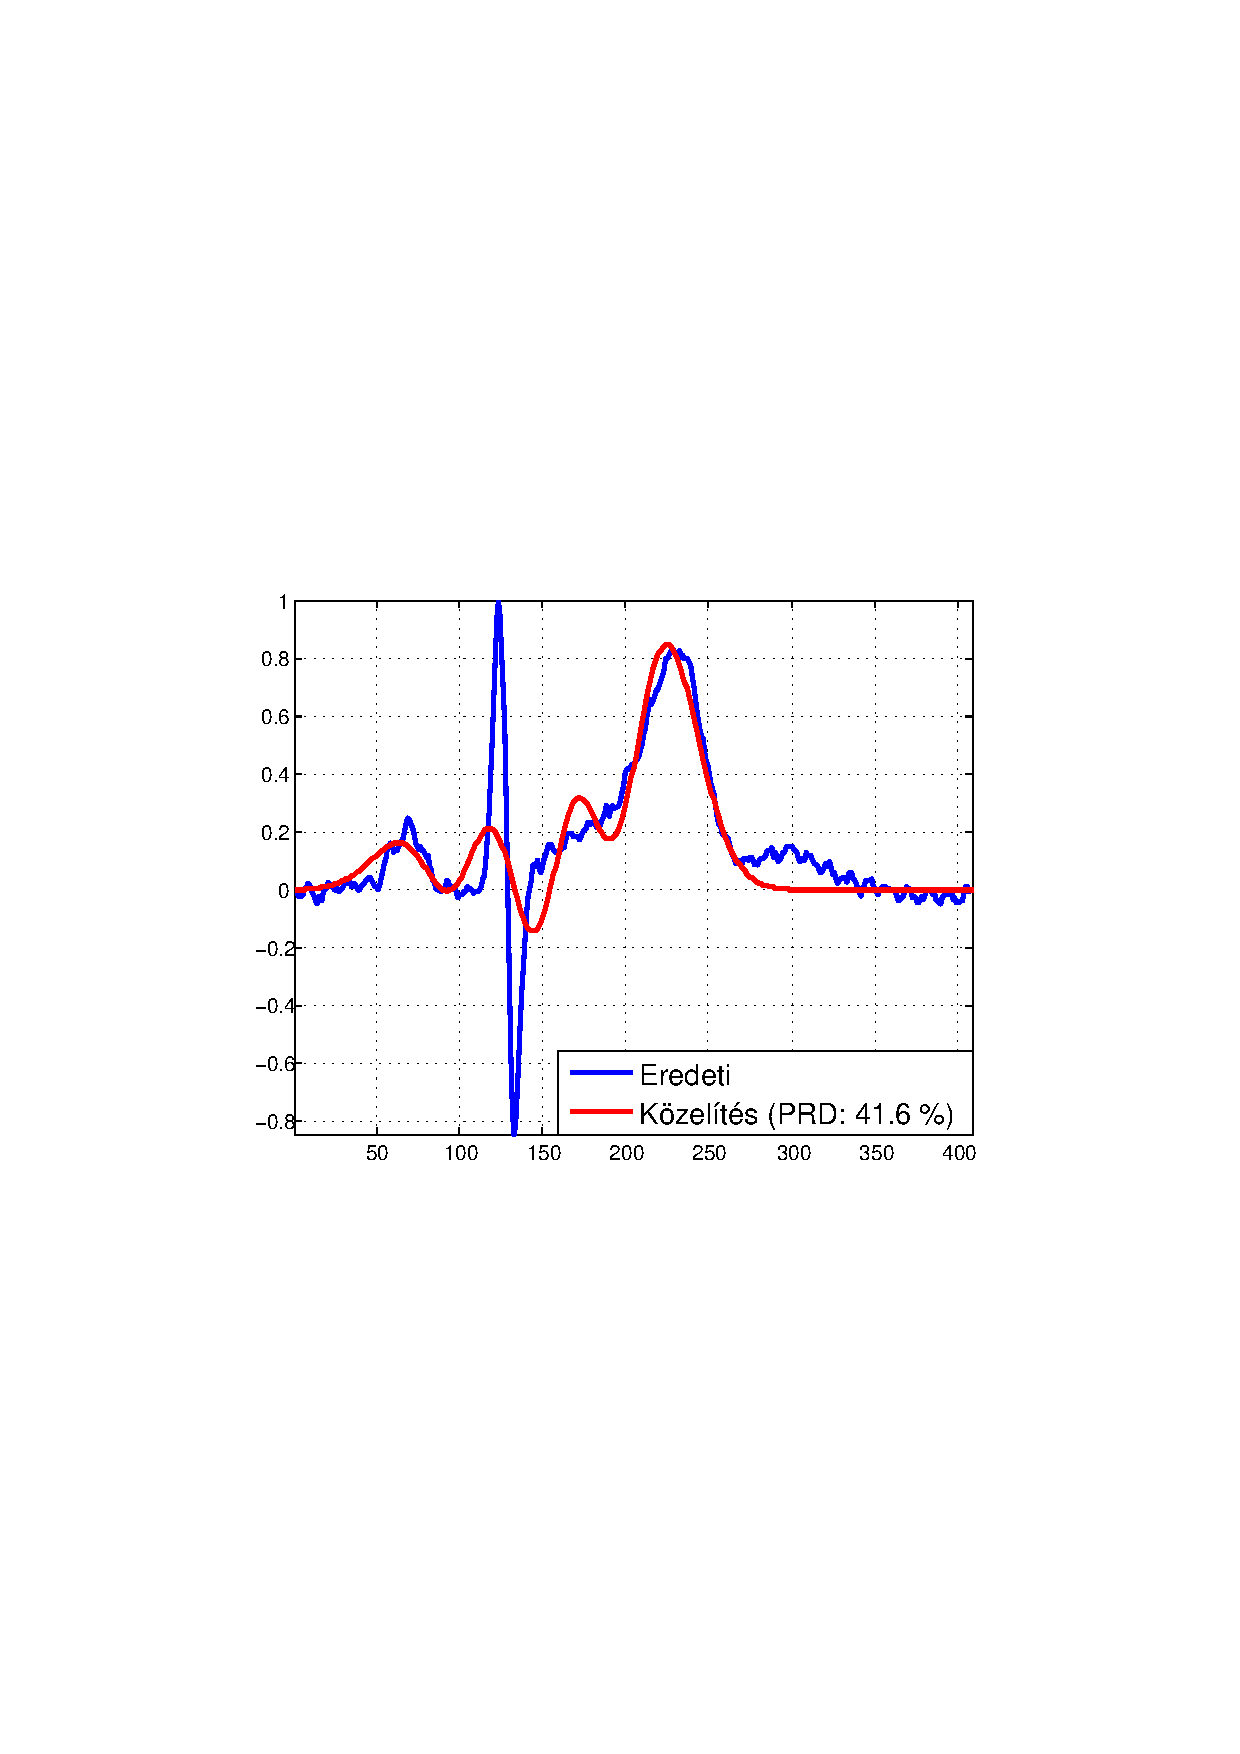
\includegraphics[scale=0.5,trim=100 280 100 280,clip]{./Abrak/Kitekintes/abra762_bad.pdf}}
\subfigure[Jó eset.]{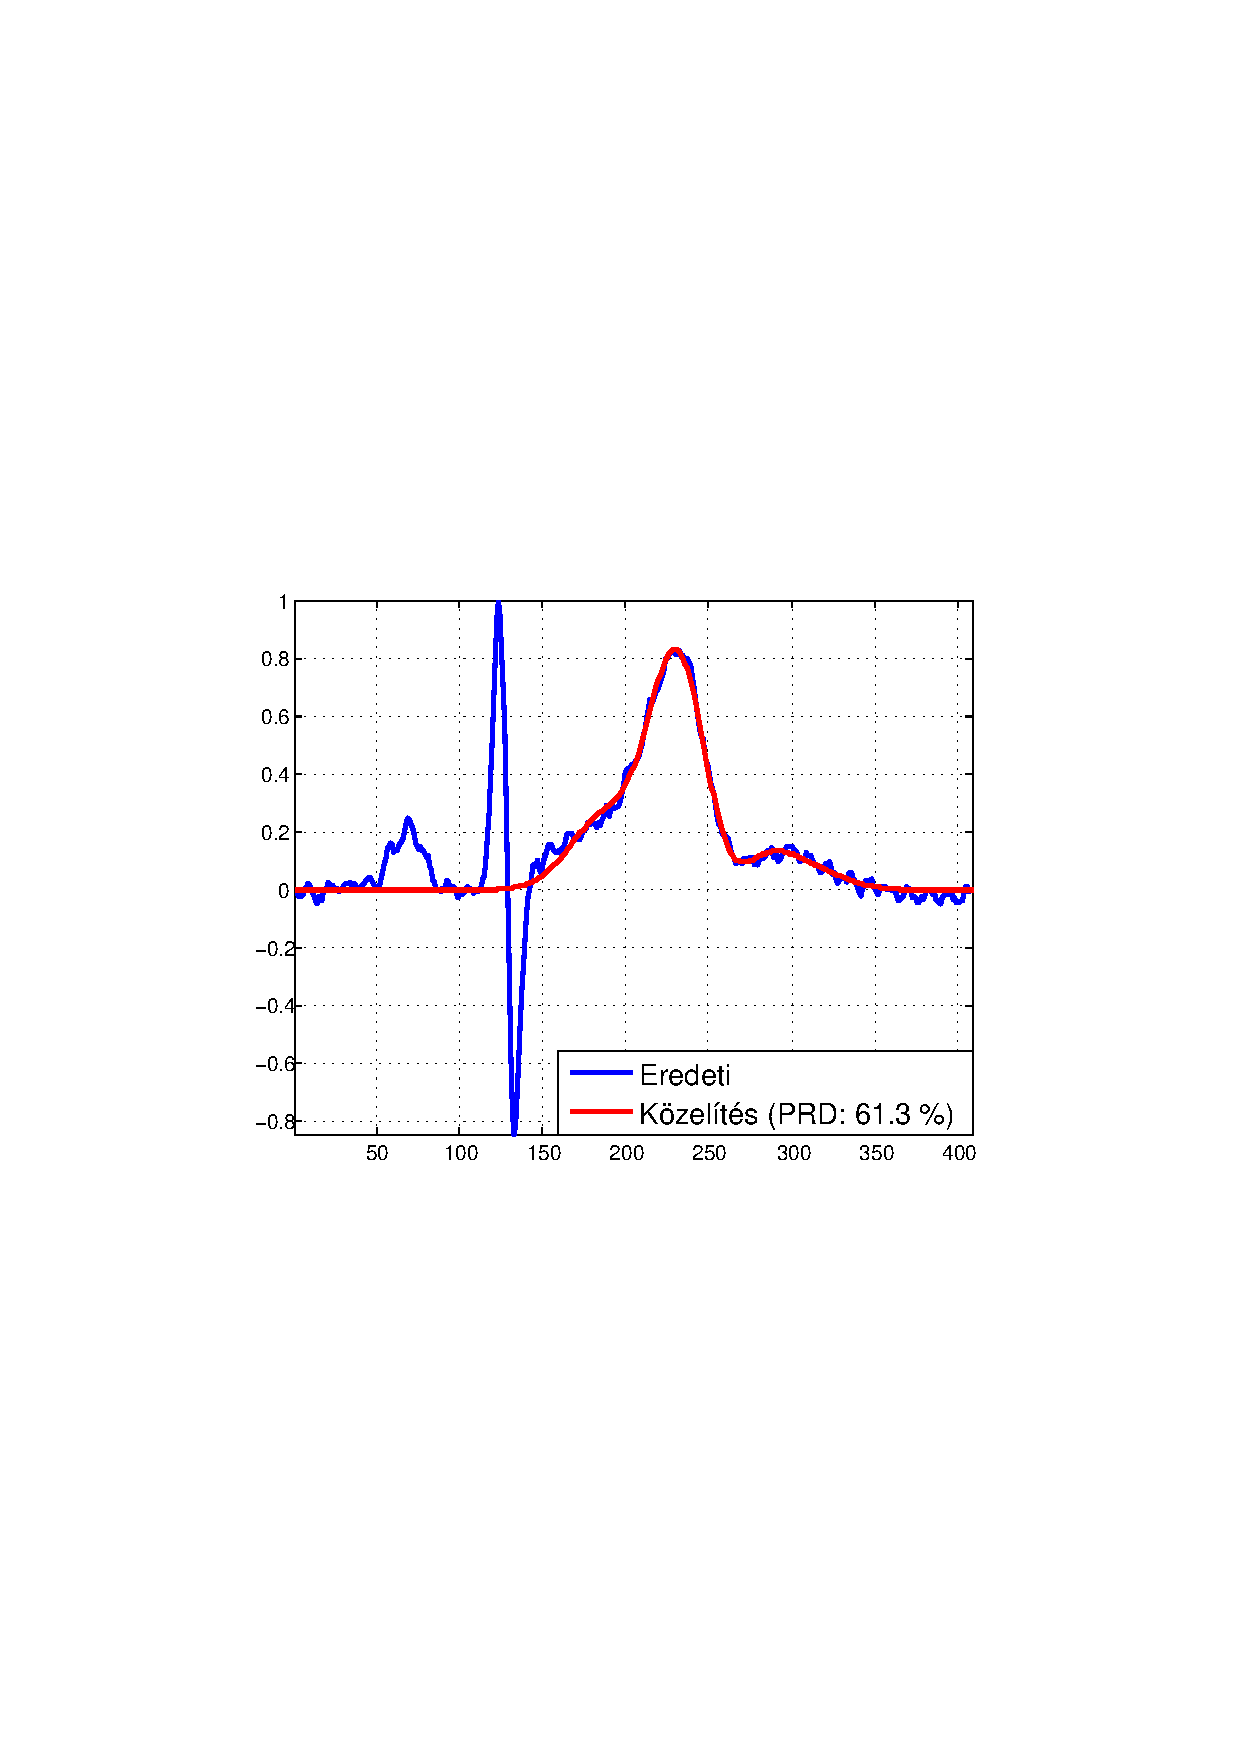
\includegraphics[scale=0.5,trim=100 280 100 280,clip]{./Abrak/Kitekintes/abra762_good.pdf}}
\caption{A mohó stratégia hátránya.}
\label{fig:counterexample}
\end{figure}	

\section*{K\"osz\"onetnyilv\'an\'\i t\'as}

K\"osz\"on\"om t\'emavezet\H omnek, Kov\'acs P\'eternek a
kitart\'o, \'es folyamatos hozz\'aj\'arul\'as\'at, \'utmutat\'as\'at. 
Szint\'en k\"osz\"on\"om a Schipp Ferenc professzor emeritusztól kapott sok \'ertekes seg\'\i ts\'eget.   
N\'elk\"ul\"uk ez a dolgozat nem j\"ohetett volna l\'etre.


%%%%%%%%%%%%%%%%%%%%%%%%%%%%%%%%%%%%%%%%%
%%%%%%%%  Függelék  %%%%%%%%%%%%%%%%%%%%%
%%%%%%%%%%%%%%%%%%%%%%%%%%%%%%%%%%%%%%%%%
\appendix
\appendixpage
\addappheadtotoc
%\section{F\"uggel\'ek}
\chapter{Definíciók, összefüggések}

Ez a fejezet a felhaszn\'alt matematikai eszk\"oz\"ok \"osszefoglal\'as\'at tartalmazza az \cite{szego, szoke} k\"onyveket alapul v\'eve.

\section {Hermite  polinomok, Hermite f\"uggv\'enyek}
\subsubsection{Stirling  formula}
\begin{equation*}
n!\thicksim \sqrt {2\pi n}\Big(\frac ne\Big)^n,  \binom {2n} n\thicksim \frac {2^{2n}}{\sqrt{\pi n}}\ \ (
n\to\infty)
\end{equation*}

\subsubsection{\it  Rodrigues formula}
\begin{equation}
\begin{split}
&H_n(x):=e^{x^2}(-1)^n\left(\frac d{dx}\right)^n e^{-x^2}\ \ (n\in\Bbb N, x\in\Bbb R)\\
\end{split}
\end{equation}

\subsubsection{\it  Ortogonalit\'as, norm\'alt renszer}
\begin{equation}
\begin{split}
&\int_{-\infty}^\infty e^{-x^2}H_n(x)H_m(x)\, dx=\pi^{1/2}2^n n!\, \delta_{mn}\ \ (m,n\in\Bbb N)\\
&\Phi_n(x):=H_n(x)e^{-x^2/2}/\sqrt{\pi^{1/2}2^n n!}=h_n(x)e^{-x^2/2} \ \ (n\in\Bbb N, x\in\Bbb R)\\
&\int_{-\infty}^\infty \Phi_n(x)\Phi_m(x)\, dx=\, \delta_{mn}\ \ (m,n\in\Bbb N)\\
&\int_{-\infty}^\infty e^{-x^2}\, dx=\pi^{1/2}<2
\end{split}
\end{equation}

\subsubsection{\it  Rekurzi\'ok}
\begin{equation}
\begin{split}
&H_n(x)=2xH_{n-1}(x)-2(n-1)H_{n-2}(x)\ (n\ge 2)\\
&H_{-1}(x)=0,  H_0(x)=1,\ \ H_1(x)=2x\\
&\Phi_n(x)=\sqrt{\frac 2 n}x\Phi_{n-1}-\sqrt{\frac {n-1} n}\Phi_{n-2}(x)\ (n\ge 2)\\ &\Phi_0(x)=e^{-x^2/2}/\pi^{1/4}, \Phi_1(x)= \sqrt 2 x e^{-x^2/2}/\pi^{1/4}\ \ (x\in\Bbb R)\\
&H'_n(x)=2nH_{n-1}(x)\ (n\in\Bbb N)\\
&\Phi'_n(x)=\sqrt{2n}\Phi_{n-1}(x)-x\Phi_n(x)\ \ (n\ge 0, x\in\Bbb R)\\
&\frac d{dx}(x\Phi_n(x))=(1-x^2)\Phi_n(x)+\sqrt{2n}x\Phi_{n-1}(x)\ \ (n\ge 1, x\in\Bbb R)
\label{eq:identities}
\end{split}
\end{equation}

\subsubsection{\it  F\"uggv\'eny\'ert\'ekek a $0$ helyen}
\begin{equation}
\begin{split}
&H_{2m+1}(0)=0,\ H_{2m}(0)=(-1)^m\frac{(2m)!}{m!}\\
&H'_{2m}(0)=0,\ H'_{2m+1}(0)=(-1)^m\frac{(2m+2)!}{(m+1)!}\\
&\Phi_{2m}(0)=(-1)^m2^{-m}\sqrt{\binom {2m}m}\thicksim (2 m)^{-1/4}\pi^{-1/2}\\
&\Phi'_{2m+1}(0)=(-1)^m2^{-m}\sqrt{\binom {2m}m}\thicksim (8m)^{1/4}\pi^{-1/2}
\end{split}
\end{equation}

\subsubsection{\it Kvadrat\'ura formula}
$$
\int_{-\infty}^\infty e^{-x^2}f(x)\, dx\backsimeq \sum_{i=1}^n \lambda_{in}f(x_{in})
$$

$$
H_n(x_{in})=0,\ \lambda_{in}=\frac{\pi^{1/2}2^{n+1}n!}{[H'_n(x_{in}]^2}\ \ \  (n=1,2,\cdots, 1\le i\le n)
$$

\section{Approxim\'aci\'o afffin transzform\'altakkal}
\label{app:aprx}

Jel\"olj\"uk az $\Bbb R$ sz\'amegyenesen szakaszonk\'ent folytonos, n\'egyzetesen integr\'alhat\'o f\"uggv\'enyek ter\'et $\mathcal F$-fel \'es vezess\"uk be az $\mathcal F$ t\'eren az
$$
\langle f,g\rangle:=\int_{-\infty}^\infty  f(x)g(x)\,dx
$$
skal\'aris szorzatot.


\subsubsection{\it  Alt\'ert\H ol vett t\'avols\'ag}

A  $\phi_n\in \mathcal F$ $(n\in\Bbb N)$ f\"uggv\'enyrendszer  ortonorm\'alt, ha
$$
\langle \phi_n,\phi_m\rangle:=\delta_{mn}\ \ (m,n\in\Bbb N).
$$
Ebb\H ol a rendszerb\H ol az
$$
\ell(x)=\ell(x,\lambda, a)=\lambda x+a\ \ (x,a\in\Bbb R,\lambda>0)
$$
affin transzform\'aci\'oval sz\'armaztatott
$$
\phi_n^{a,\lambda}(x):=\sqrt \lambda \phi_n(\lambda x+a)=\sqrt \lambda \phi_n(\ell(x)) \ (x,a\in\Bbb R,\lambda>0, n\in\Bbb N)
$$
rendszer szint\'en ortonorm\'alt. Val\'oban az $u=\ell(x)=\lambda x+a, dx=du/\lambda $ helyettes\'\i t\'essel
\begin{equation}
\begin{split}
&\langle \phi_n^{a,\lambda},\phi_m^{a,\lambda}\rangle:=
\int_{-\infty}^\infty\lambda \phi_n(\lambda x+a)\phi_m(\lambda x+a)\, dx=\\
&=\int_{-\infty}^\infty \phi_n(u)\phi_m(u)\, dx=
\delta_{mn}\ \ (m,n\in\Bbb N).
\end{split}
\end{equation}
Jel\"olje  $X_n^{a,\lambda}$ a $\phi_0^{a,\lambda},\cdots,\phi_n^{a,\lambda}$ f\"uggv\'enyek \'altal kifesz\'\i tett alteret. Adott $f\in \mathcal F$ fuggv\'enyhez a legk\"ozelebb es\H o $X_n^{a,\lambda}$-beli f\"uggv\'enyt az
$$
S_n^{a,\lambda}f:=\sum_{k=0}^n \langle f,\phi_n^{a,\lambda}\rangle\phi_n^{a,\lambda}
$$
Fourier-projekci\'oval, az elt\'er\'es norm\'aj\'anak a  n\'egyzete  a
$$
D_n^2(a,\lambda):=\|f-S_n^{a,\lambda}f\|^2=\langle f,f\rangle-\sum_{k=0}^n |\langle f,\phi_k^{a,\lambda}\rangle|^2
$$
f\"uggv\'ennyel adhat\'o meg. A $D_n(a,\lambda)$ minimum\'anak meghat\'aroz\'asa ekvivalens az
$$
F_n(a,\lambda):=\sum_{k=0}^n |\langle f,\phi_k^{a,\lambda}\rangle|^2\ \
((a,\lambda)\in T:=\{(p,q)\in\Bbb R^2:p\in\Bbb R, q>0\}
$$
f\"uggv\'eny maximum\'anak meghat\'aroz\'as\'aval.

\subsubsection{\it  Becsl\'esek az $F_n$ f\"uggv\'enyre}

 A tov\'abbiakban a
 $$
 \phi_n(x)=\Phi_n(x)=h_n(x)e^{-x^2/2}\ \ (x\in\Bbb R, n\in\Bbb N)
 $$
 norm\'alt Hermite-f\"uggv\'enyeket v\'alasztjuk ortonorm\'alt rendszernek. Ekkor
 \begin{equation}
 \begin{split}
 &|\Phi_n(x)|\le M_n e^{-x^2/4}\le M_n, \ |\Phi_n'(x)|\le N_n e^{-x^2/4}\le N_n\ (x\in\Bbb R, n\in\Bbb N)\\
 &M_n:=\max_{x\in\Bbb R}|h_n(x)|e^{-x^2/4},\ N_n:=\max_{x\in\Bbb R}|h'_n(x)-xh_n(x)|e^{-x^2/4}\\
 &\int_{-\infty}^\infty|\Phi_n(x)|\, dx\le M_n\int_{-\infty}^\infty e^{-x^2/4}\, dx<4M_n
 \end{split}
 \end{equation}
 Ezeket felhaszn\'alva becsl\'eseket adunk az
 $$
 A_k(a,\lambda):=\langle f,\phi_k^{a,\lambda}\rangle=\sqrt{\lambda}\int_{-\infty}^\infty f(x)\phi_k(\lambda x+a)\, dx=\frac 1{\sqrt{\lambda}}\int_{-\infty}^\infty f((u-a)/\lambda)\phi_k(u)\, du
 $$
 Fourier-egy\"utthat\'okra. A tov\'abbiakban kompakt tart\'oj\'u, korl\'atos f\"uggv\'enyekb\H ol indulunk ki. Nem jelenti az \'altal\'anoss\'ag megszor\'\i t\'as\'at ha  feltessz\"uk, hogy
 $$
 f(x)=0,\ \text{ha}\ |x|\ge 1,\ \ |f(x)|\le 1 \ (x\in\Bbb R).
 $$
 A param\'eteres integr\'alokra vonatkoz\'o t\'etelb\H ol  k\"ovetkezik, hogy   az
 $$
 F_n(a,\lambda):=\sum_{k=0}^n|A_k(a,\lambda)|^2\ \ \  ((a,\lambda)\in T>0)
 $$
 f\"uggv\'eny folytonosan  differenci\'alhat\'o. Megmutatjuk, hogy az $F_n:T\to [0,\infty)$
 folytonos f\"uggv\'enynek van maximuma a $T$ (nem kompakt) halmazon.

 A fenti egyenl\H otlens\'egekb\H ol k\"ovetkezik, hogy
 \begin{equation}
 \begin{split}
 &|A_k(\lambda,a)|\le \sqrt{\lambda} M_k\int_{-\infty}^\infty |f(x)|\, dx\le 2M_k\sqrt{\lambda}\ \ (\lambda\le 1)\\
 &|A_k(\lambda,a)|\le\frac 1{\sqrt{\lambda}}\int_{-\infty}^\infty |\Phi_k(u)|\, du\le
 \frac {4M_k}{\sqrt{\lambda}}\ (\lambda\ge 1),
 \end{split}
 \end{equation}
 tov\'abb\'a $\lambda\ge 1,\ a\ge 2\lambda $ eset\'en
 \begin{equation}
 \begin{split}
 &|A_k(\lambda,a)|\le \frac 1{\sqrt{\lambda}}\int_{a-\lambda}^{a+\lambda}|\Phi_k(u)|\, du
 \le \frac 1{\sqrt{\lambda}}\int_{a-\lambda}^\infty |\Phi_k(u)|\, du\le\\
 &\le \frac {M_k}{\sqrt{\lambda}}\int_\lambda^\infty e^{-{u^2}/4}\, du<
 \frac {M_k}{\sqrt{\lambda}}\int_\lambda^\infty u e^{-{u^2}/4}\, du=
 2 M_k\sqrt{\lambda} e^{-{\lambda^2}/4}<\frac {8M_k}{\sqrt{\lambda}}
\end{split}
\end{equation}
Hasonl\'oan egyenl\H otlens\'eget kapunk az $a<-2\lambda$ esetben. Innen k\"ovetkezik, hogy az
$$
T_s:=\{(p,q): -2s\le p\le 2s, 1/s\leq p \le s\}
$$
t\'eglalapon k\'\i v\"ul  \'erv\'enyes
$$
\sup_{(a,\lambda) \notin T_s}|A_k(a,\lambda)|\le \frac {8M_k}{\sqrt s}\ \  (s>1)
$$
becsl\'es. Ennek alapj\'an nyilv\'anval\'o, hogy a $F_n$  f\"uggv\'enynek l\'etezik a maximuma a $T$ t\'eglelapon.


C\'elunk az
 maximum meghat\'aroz\'asa a leggyorsabb ereszked\'es elve alapj\'an. Bevezetve az $s(u)=\ell^{-1}(u)=(u-a)/\lambda$ jel\"ol\'est, a  param\'eteres integr\'al differenci\'al\'asi szab\'alya alapj\'an  azt kapjuk, hogy
\begin{equation}
\begin{split}
&\frac \partial {\partial a}A_k(a,\lambda)=\lambda^{1/2} \int_{-\infty}^\infty f(x)\phi_k'(\ell(x))\, dx\\
 &\frac \partial {\partial \lambda}A_k(a,\lambda)=\lambda^{1/2} \int_{-\infty}^\infty f(x)x\phi_k'(\ell(x))\, dx+\frac 12\lambda^{-1/2}\int_{-\infty}^\infty f(x)\phi_k(\ell(x))
 \end{split}
 \end{equation}

 A parci\'alis deriv\'altak a k\"ovetkez\H o h\'arom sorozattal fejezehet\H ok ki:
 \begin{equation}
 \begin{split}
 &A_k(a,\lambda):=\sqrt{\lambda}\int_{-\infty}^\infty f(x)\phi_k(\ell(x))\, dx\\
 &A_k^{[1]}(a,\lambda):=\sqrt{\lambda}\int_{-\infty}^\infty f(x))\phi_k'(\ell(x))\, dx\\
 &A_k^{[2]}(a,\lambda):=\sqrt{\lambda}\int_{-\infty}^\infty xf(x))\phi_k'(\ell(x))\, dx.
 \end{split}
  \end{equation}
Nevezetesen
\begin{equation}
\begin{split}
&F(a,\lambda)=\sum_{k=0}^n A_k^2(a,\lambda)\\
&\frac 12\frac \partial{\partial a} F(\lambda, a)=\sum_{k=0}^n A_k(a,\lambda)A_k^{[1]}(a,\lambda)\\
&\frac 12\frac \partial{\partial \lambda} F(a,\lambda)=\frac 1{2\lambda}\sum_{k=0}^n A_k^2(a,\lambda)+\sum_{k=0}^n A_k(\lambda,a)A_k^{[2]}(a,\lambda)=\\
&=\frac 1{2\lambda} F(a,\lambda )+\sum_{k=0}^n A_k(\lambda,a)A_k^{[2]}(\lambda,a)
\end{split}
\end{equation}

\chapter{Algoritmusok}
\label{chp:alg}
%\section{PSO pszeudok\'od}
\begin{algorithm}[htp] 
\begin{algorithmic}[1]
	\Function{PSO}{$Hiba,\,S,\,I_N,c_{1,2}$} 		
	\ForAll{$k\gets 1, S$} %\Comment{In our case, $c_1=1.5,\,c_2=2$ and $V_{max}=0.5\,.$}
		\State Randomize $\lambda_k,\; a_k, \; v_k$	 		
		\State Initialize $H_k.\lambda:=\lambda_k$ \Comment{A r\'eszecsk\'ehez tartoz\'o dilat\'aci\'o}
		\State Initialize $H_k.a:=a_k$		\Comment{A r\'eszecsk\'ehez tartoz\'o transzl\'aci\'o}	
		\State Initialize $H_k.pBest:=[\lambda_k, a_k]$    \Comment{A r\'eszecske legjobb poz\'\i ci\'oja}
		\State Initialize $H_k.pDBest:=\infty$   \Comment{A r\'eszecske legkisebb hib\'aja}
		\State Initialize $H_k.v:=v_k$   \Comment{A r\'eszecske kezd\H o gyorsul\'asa}
	\EndFor
	\For{$\ell\gets 1, I_N$}	
		\For{$k\gets 1, S$}								
			\If{$Hiba(H_k)<H_k.pDBest$}  \Comment{pBest friss\'\i t\'ese}
				\State $H_k.pBest=[\lambda_k, a_k]$
				\State $H_k.pDBest= Hiba(H_k)$
			\EndIf
		\EndFor		
		\If{$Hiba(H_k)<\underset{1\leq k\leq S}{\min}\, Hiba(H_k)$}  \Comment{gBest friss\'\i t\'ese}
				\State $gBest=[H_k.\lambda, H_k.a]$
			\EndIf

	\For{$k\gets 1, S$}						\Comment{gyorsul\'as \'es poz\'\i ci\'o friss\'\i t\'ese}
			\State $H_k.v = H_k.v + c_1 r_1 \cdot (H_k.pBest-[\lambda_k, a_k]) 
						 + c_2 r_2 \cdot (gBest-[\lambda_k, a_k])$ 
			\State $H_k.\lambda = H_k.\lambda + H_k.v$	
			\State $H_k.a = H_k.a + H_k.v$
			
		\EndFor					
	\EndFor
	\State \textbf{return} $gBest$
	\EndFunction
\end{algorithmic}
\caption{Particle Swarm Optimization}
\label{alg:pso}
\end{algorithm}
\newpage
%\section{Nelder-Mead pszeudok\'od}
Az indexeket \'ugy rendezz\"uk, hogy
$y_3\le y_2\le y_1$ teljes\"ulj\"on. Az $IterLepes(5)$ rutinnal az 
$(x_1,x_2,x_3)$ h\'armast kicser\'elj\"uk a $T_5$ transzform\'aci\'oval kapott
h\'armassal.
\bigskip

\begin{algorithm}[htb!] 
\begin{algorithmic}[1]
	\Function{Nelder-Mead}{} 
	\If{$y_3 \leq y_4 \wedge y_4 < y_2$}
		\State $x_1 = x_4$
	\ElsIf{$y_4 < y_3$}
		\If{$y_5 < y_4$}
			\State $x_1 = x_5$
		\Else
			\State $x_1 = x_4$
		\EndIf
	\ElsIf{$y_4 \geq y_2$}
		\If{$y_4 < y_1$}
			\If{$y_6 \leq y_4$}
				\State $x_1 = x_6$
			\Else
				\State $IterLepes(5)$
			\EndIf
		\ElsIf{$y_4 \geq y_1$}
			\If{$y_7 < y_3$}
				\State $x_1 = x_7$
			\Else
				\State $IterLepes(5)$
			\EndIf
		\EndIf
	\EndIf
	\EndFunction
\end{algorithmic}
\caption{Nelder-Mead}
\label{alg:NM}
\end{algorithm}

% \begin{center}
%  \begin{tabular}{cc}
  %  \includegraphics[width=50mm]{HaarR1.pdf}
  %  \includegraphics[width=50mm]{HaarR2.pdf}
%  \end{tabular}

%  $h_m\ (m=0,1,\cdots,7)\ \ \ \ \ \ \ \ \ \ \ \ \ S_{2^n}^Hf\ (n=2, 3,4)$
%\end{center}
% \goodbreak

%----------------------------REFERENCES
\bibliographystyle{IEEEbib}
\bibliography{refs}


\end{document}
%%%%%%%%%%%%%%%%%%%%%%%%%%%%%%%%%%%%%%%%%%%%%%%%%%%%%%%%%%%%%%%%%%%%%%%%%%%%%%%%%%%%%%%%%%%%
